%%%%%%%% ICML 2019 EXAMPLE LATEX SUBMISSION FILE %%%%%%%%%%%%%%%%%

\documentclass{article}

% Recommended, but optional, packages for figures and better typesetting:
\usepackage{microtype}
\usepackage{graphicx}
\usepackage{subfigure}
\usepackage{booktabs} % for professional tables
\usepackage[noend]{algpseudocode}
\usepackage{amsthm,amssymb,amsmath}
\usepackage{amsmath}
\usepackage{glossaries}
\usepackage{listings}

% hyperref makes hyperlinks in the resulting PDF.
% If your build breaks (sometimes temporarily if a hyperlink spans a page)
% please comment out the following usepackage line and replace
% \usepackage{icml2019} with \usepackage[nohyperref]{icml2019} above.
\usepackage{hyperref}
% Attempt to make hyperref and algorithmic work together better:
\newcommand{\theHalgorithm}{\arabic{algorithm}}

\newtheorem{theorem}{Theorem}
\newtheorem{corollary}{Corollary}
%\newtheorem{lemma}[theorem]{Lemma}
\newtheorem{lemma}{Lemma}

\DeclareMathOperator*{\argmin}{argmin}
\DeclareMathOperator*{\argmax}{argmax}

% Use the following line for the initial blind version submitted for review:
%\usepackage{icml2019}

\newcommand{\adam}[1]{\textbf{\textcolor{magenta}{#1}}}
\newcommand{\noam}[1]{\textbf{\textcolor{cyan}{#1}}}

% If accepted, instead use the following line for the camera-ready submission:
\usepackage[accepted]{icml2019}

% The \icmltitle you define below is probably too long as a header.
% Therefore, a short form for the running title is supplied here:
\icmltitlerunning{Deep Counterfactual Regret Minimization}

\begin{document}

\twocolumn[
\icmltitle{Deep Counterfactual Regret Minimization}

% It is OKAY to include author information, even for blind
% submissions: the style file will automatically remove it for you
% unless you've provided the [accepted] option to the icml2019
% package.

% List of affiliations: The first argument should be a (short)
% identifier you will use later to specify author affiliations
% Academic affiliations should list Department, University, City, Region, Country
% Industry affiliations should list Company, City, Region, Country

% You can specify symbols, otherwise they are numbered in order.
% Ideally, you should not use this facility. Affiliations will be numbered
% in order of appearance and this is the preferred way.
\icmlsetsymbol{equal}{*}

\begin{icmlauthorlist}
\icmlauthor{Noam Brown}{equal,cmu,fair}
\icmlauthor{Adam Lerer}{equal,fair}
\icmlauthor{Sam Gross}{fair}
\icmlauthor{Tuomas Sandholm}{cmu}
\end{icmlauthorlist}

\icmlaffiliation{fair}{Facebook AI Research}
\icmlaffiliation{cmu}{Computer Science Department, Carnegie Mellon University}

\icmlcorrespondingauthor{Noam Brown}{noamb@cs.cmu.edu}

% You may provide any keywords that you
% find helpful for describing your paper; these are used to populate
% the "keywords" metadata in the PDF but will not be shown in the document
\icmlkeywords{CFR, Counterfactual Regret Minimization, Deep Reinforcement Learning, Poker, Regret Minimization, No-Regret Learning, Deep Learning}

\vskip 0.3in
]

% this must go after the closing bracket ] following \twocolumn[ ...

% This command actually creates the footnote in the first column
% listing the affiliations and the copyright notice.
% The command takes one argument, which is text to display at the start of the footnote.
% The \icmlEqualContribution command is standard text for equal contribution.
% Remove it (just {}) if you do not need this facility.

%\printAffiliationsAndNotice{}  % leave blank if no need to mention equal contribution
\printAffiliationsAndNotice{\icmlEqualContribution} % otherwise use the standard text.

\begin{abstract}
\vspace{-0.03in}
\emph{Counterfactual Regret Minimization (CFR)} is the leading framework for solving large imperfect-information games. %It iteratively traverses the game tree in order to converge to an equilibrium.
It converges to an equilibrium by iteratively traversing the game tree.
%In order to deal with extremely large games, CFR typically uses domain-specific heuristics to simplify the target game in a process known as \emph{abstraction}.
In order to deal with extremely large games, abstraction is typically applied before running CFR. The abstracted game is solved with tabular CFR, and its solution is mapped back to the full game. This process can be problematic because aspects of abstraction are often manual and domain specific, abstraction algorithms may miss important strategic nuances of the game, and there is a chicken-and-egg problem because determining a good abstraction requires knowledge of the equilibrium of the game.
This paper introduces \emph{Deep Counterfactual Regret Minimization}, a form of CFR that obviates the need for abstraction by instead using deep neural networks to approximate the behavior of CFR in the full game. We show that Deep CFR is principled and achieves strong performance in large poker games. This is the first non-tabular variant of CFR to be successful in large games.
\end{abstract}

\section{Introduction}
\vspace{-0.03in}
\label{sec:intro}

Imperfect-information games model strategic interactions between multiple agents with only partial information. They are widely applicable to real-world domains such as negotiations, auctions, and cybersecurity interactions. Typically in such games, one wishes to find an approximate equilibrium in which no player can improve by deviating from the equilibrium.

%Due to the presence of multiple agents whose strategies may not be stationary, imperfect-information games cannot be solved using methods that are used for partially observable Markov decisions processes. Likewise, due to the presence of hidden information, search-based techniques such as Monte Carlo Tree Search are ineffective both in theory and in practice for imperfect-information games. For these reasons, a different approach is required.

The most successful family of algorithms for imperfect-information games have been variants of \emph{Counterfactual Regret Minimization (CFR)}~\cite{Zinkevich07:Regret}. CFR is an iterative algorithm that converges to a Nash equilibrium in two-player zero-sum games. Forms of tabular CFR have been used in all recent milestones in the benchmark domain of poker~\cite{Bowling15:Heads-up,Moravcik17:DeepStack,Brown17:Superhuman} and have been used in all competitive agents in the Annual Computer Poker Competition going back at least six years.\footnote{\href{www.computerpokercompetition.org}{www.computerpokercompetition.org}} In order to deal with extremely large imperfect-information games, \emph{abstraction} is typically used to simplify a game by bucketing similar states together and treating them identically. The simplified (abstracted) game is approximately solved via tabular CFR. However, constructing an effective abstraction requires extensive domain knowledge and the abstract solution may only be a coarse approximation of a true equilibrium.

In constrast, reinforcement learning has been successfully extended to large state spaces by using function approximation with deep neural networks rather than a tabular representation of the policy (deep RL). This approach has led to a number of recent breakthroughs in constructing strategies in large MDPs~\cite{Mnih15:Human} as well as in zero-sum perfect-information games such as Go~ \cite{Silver17:Mastering,Silver18:General}.\footnote{Deep RL has also been applied successfully to some partially observed games such as Doom~\cite{lample2017playing}, as long as the hidden information is not too strategically important.} Importantly, deep RL can learn good strategies with relatively little domain knowledge for the specific game~\cite{Silver17:Mastering}.
%Recent work has also combined deep RL with Monte Carlo Tree Search as a policy improvement operator to improve the performance of RL training \cite{silver2017mastering}.
However, most popular RL algorithms do not converge to good policies (equilibria) in imperfect-information games in theory or in practice.
%CFR is the leading algorithm for finding equilibrium strategies in partial information games, but currently requires a tabular strategy representation and the state space must be reduced with hand-designed abstractions\cite{libratus}.

Rather than use tabular CFR with abstraction, this paper introduces a form of CFR, which we refer to as \emph{Deep Counterfactual Regret Minimization}, that uses function approximation with deep neural networks to approximate the behavior of tabular CFR on the full, unabstracted game. We prove that Deep CFR converges to an $\epsilon$-Nash equilibrium in two-player zero-sum games and empirically evaluate performance in poker variants, including heads-up limit Texas hold'em. We show Deep CFR outperforms Neural Fictitious Self Play (NFSP)~\cite{Heinrich16:Deep}, which was the prior leading function approximation algorithm for imperfect-information games, and that Deep CFR is competitive with domain-specific tabular abstraction techniques.

%\adam{We prove that Deep CFR converges to an $\epsilon$-Nash equilibrium in IIGs. We evaluate Deep CFR in two variants of poker: X and Y. We observe performance in X comparable to abstractions used in ACPC. In Y, we XXX.}

\section{Notation and Background}
\vspace{-0.03in}
\label{sec:background}
In an imperfect-information extensive-form (that is, tree-form) game there is a finite set of players, $\mathcal{P}$. A \emph{node} (or history) $h$ is defined by all information of the current situation, including private knowledge known to only one player. $A(h)$ denotes the actions available at a node and $P(h)$ is either chance or the unique player who acts at that node. If action $a \in A(h)$ leads from $h$ to $h'$, then we write $h \cdot a = h'$. We write $h \sqsubset h'$ if a sequence of actions leads from $h$ to $h'$. $H$ is the set of all nodes.
$Z \subseteq H$ are terminal nodes for which no actions are available. For each player $p \in \mathcal{P}$, there is a payoff function $u_p: Z\rightarrow \mathbb{R}$. 
In this paper we assume $\mathcal{P} = \{1, 2\}$ and $u_1 = -u_2$ (the game is two-player zero-sum).
We denote the range of payoffs in the game by $\Delta$.

Imperfect information is represented by {\em information sets} (infosets) for each player $p \in \mathcal{P}$. For any infoset $I$ belonging to $p$, all nodes $h, h' \in I$ are indistinguishable to $p$. Moreover, every non-terminal node $h \in H$ belongs to exactly one infoset for each $p$. We represent the set of all infosets belonging to $p$ where $p$ acts by $\mathcal{I}_p$. We call the set of all terminal nodes with a prefix in $I$ as $Z_I$, and we call the particular prefix $z[I]$. We assume the game features \emph{perfect recall}, which means if $h$ and $h'$ do not share a player $p$ infoset then all nodes following $h$ do not share a player $p$ infoset with any node following $h'$.

A strategy (or policy) $\sigma(I)$ is a probability vector over actions for acting player~$p$ in infoset $I$. Since all states in an infoset belonging to $p$ are indistinguishable, the strategies in each of them must be identical. The set of actions in $I$ is denoted by $A(I)$. The probability of a particular action $a$ is denoted by $\sigma(I,a)$.
We define $\sigma_p$ to be a strategy for $p$ in every infoset in the game where $p$ acts.
A strategy profile $\sigma$ is a tuple of strategies, one for each player. The strategy of every player other than $p$ is represented as $\sigma_{-p}$. $u_p(\sigma_p, \sigma_{-p})$ is the expected payoff for $p$ if player $p$ plays according to $\sigma_p$ and the other players play according to $\sigma_{-p}$.

$\pi^{\sigma}(h) = \Pi_{h' \cdot a \sqsubseteq h} \sigma_{P(h')}(h',a)$ is called {\em reach} and is the probability $h$ is reached if all players play according to $\sigma$. $\pi^{\sigma}_p(h)$ is the contribution of $p$ to this probability.
%(that is, the probability of reaching $h$ if chance and all players other than $p$ always choose actions leading to $h$, but $p$ plays according to $\sigma_p$) \adam{I think this parenthetical is unnecessary}.
$\pi^{\sigma}_{-p}(h)$ is the contribution of chance and all players other than $p$.
%(that is, the probability of reaching $h$ if $p$ chooses actions leading toward $h$, but chance and all players other than $p$ play according to $\sigma_{-p}$ \adam{unnecessary}).
For an infoset $I$ belonging to $p$, the probability of reaching $I$ if $p$ chooses actions leading toward $I$ but chance and all players other than $p$ play according to $\sigma_{-p}$ is denoted by $\pi^{\sigma}_{-p}(I) = \sum_{h \in I}\pi^{\sigma}_{-p}(h)$.
For $h \sqsubseteq z$, define $\pi^\sigma(h \to z) = \Pi_{h' \cdot a \sqsubseteq z,h'\not\sqsubset h} \sigma_{P(h')}(h',a)$ 
%\adam{This quantity is referred to as the {\it counterfactual reach}.}

A {\em best response} to $\sigma_{-p}$ is a player~$p$ strategy $BR(\sigma_{-p})$ such that $u_p\big(BR(\sigma_{-p}), \sigma_{-p}\big) = \max_{\sigma'_p} u_p(\sigma'_p, \sigma_{-p})$.
A {\em Nash equilibrium} $\sigma^*$ is a strategy profile where everyone plays a best response: $\forall p$, $u_p(\sigma^*_p, \sigma^*_{-p}) = \max_{\sigma'_p} u_p(\sigma'_p, \sigma^*_{-p})$~\cite{Nash50:Eq}.
The {\em exploitability} $e(\sigma_p)$ of a strategy $\sigma_p$ in a two-player zero-sum game is how much worse $\sigma_p$ does versus $BR(\sigma_p)$ compared to how a Nash equilibrium strategy $\sigma^*_p$ does against $BR(\sigma^*_p)$. Formally, $e(\sigma_p) = u_p\big(\sigma_p^*,BR(\sigma_p^*)\big) - u_p\big(\sigma_p,BR(\sigma_p)\big)$. We measure \emph{total exploitability} $\sum_{p \in P} e(\sigma_p)$\footnote{Some prior papers instead measure \emph{average} exploitability rather than \emph{total} (summed) exploitability.}.
%\adam{Perhaps add a footnote mentioning that some prior work uses average exploitability}

\subsection{Counterfactual Regret Minimization (CFR)}
\vspace{-0.03in}
CFR is an iterative algorithm that converges to a Nash equilibrium in any finite two-player zero-sum game with a theoretical convergence bound of $O(\frac{1}{\sqrt{T}})$. In practice CFR converges much faster. We provide an overview of CFR below; for a full treatment, see~\citet{Zinkevich07:Regret}. Some recent forms of CFR converge in $O(\frac{1}{T^{0.75}})$ in self-play settings~\cite{Farina19:Stable}, but are slower in practice so we do not use them in this paper.

%CFR is an iterative algorithm that maintains a \adam{counterfactual?} \emph{regret} value (defined later) for each action in each infoset, and uses those values to define a strategy for each player on each iteration. Based on those strategies, CFR updates the regret values. 

Let $\sigma^t$ be the strategy profile on iteration $t$.  The \emph{counterfactual value} $v^{\sigma}(I)$ of player $p=P(I)$ at $I$ is the expected payoff to $p$ when reaching $I$, weighted by the probability that $p$ would reached $I$ if she tried to do so that iteration. Formally,
\begin{equation}
\label{def:v}
v^\sigma(I) = \sum_{z\in Z_I} \pi_{-p}^\sigma(z[I])\pi^\sigma(z[I] \to z) u_p(z)
\end{equation}
and $v^\sigma(I,a)$ is the same except it assumes that player~$p$ plays action~$a$ at infoset~$I$ with 100\% probability.

The {\em instantaneous regret} $r^t(I,a)$ is the difference between $P(I)$'s counterfactual value from playing $a$ vs. playing $\sigma$ on iteration $t$
\begin{equation}
%r^t(I,a) = \pi_{-p}^{\sigma^t}(I) \big(v^{\sigma^t}(I,a) - v^{\sigma^t}(I)\big)
r^t(I,a) = v^{\sigma^t}(I,a) - v^{\sigma^t}(I)
\label{eq:instant}
\end{equation}
The {\em counterfactual regret} for infoset $I$ action $a$ on iteration $T$ is
\begin{equation}
R^T(I,a) = \sum_{t = 1}^T r^t(I,a)
\label{eq:regret}
\end{equation}
Additionally, $R^T_+(I,a) = \max\{R^T(I,a), 0 \}$ and $R^T(I) = \max_a\{R^T(I,a)\}$. \emph{Total regret}
for $p$ in the entire game is
%\begin{equation}
$R_p^T = \max_{\sigma_p'} \sum_{t = 1}^T \big(u_p(\sigma'_p, \sigma_{-p}^t) - u_p(\sigma^t_p, \sigma_{-p}^t)\big)$.
%\end{equation}

CFR determines an iteration's strategy by applying any of several \emph{regret minimization} algorithms to each infoset~\cite{Littlestone94:Weighted,Chaudhuri09:Parameter-free}.  Typically, {\em regret matching} (RM) is used as the regret minimization algorithm within CFR due to RM's simplicity and lack of parameters~\cite{Hart00:Simple}.

In RM, a player picks a distribution over actions in an infoset in proportion to the positive regret on those actions. Formally, on each iteration $t+1$, $p$ selects actions $a \in A(I)$ according to probabilities
\begin{equation}
\sigma^{t+1}(I,a) =
\frac{R^t_+(I,a)}{\sum_{a' \in A(I)}R_+^t(I,a')}
\label{eq:rm}
\end{equation}
If $\sum_{a' \in A(I)}R_+^t(I,a') = 0$ then any arbitrary strategy may be chosen. Typically each action is assigned equal probability, but in this paper we choose the action with highest counterfactual regret with probability $1$, which we find empirically helps RM better cope with approximation error (see Figure \ref{fig:ablations}).

If a player plays according to regret matching in infoset $I$ on every iteration, then on iteration $T$, $R^T(I) \le \Delta\sqrt{|A(I)|}\sqrt{T}$~\cite{Cesa-Bianchi06:Prediction}.
\citet{Zinkevich07:Regret} show that the sum of the counterfactual regret across all infosets upper bounds the total regret. Therefore,
if player~$p$ plays according to CFR on every iteration, then
%\begin{equation}
$R_p^T \le \sum_{I \in \mathcal{I}_p} R^T(I)$.
%\label{eq:bound}
%\end{equation}
So, as $T \rightarrow \infty$, $\frac{R_p^T}{T} \rightarrow 0$.

The average strategy $\bar{\sigma}_p^T(I)$ for an infoset $I$ on iteration $T$ is
%\begin{equation}
$\bar{\sigma}_p^T(I) = \frac{\sum_{t = 1}^T \big(\pi_p^{\sigma^t}(I)\sigma_p^t(I)\big)}{\sum_{t = 1}^T \pi_p^{\sigma^t}(I)}$.
%\label{eq:average}
%\end{equation}

In two-player zero-sum games, if both players' average total regret satisfies $\frac{R_p^T}{T} \le \epsilon$, then their average strategies $\langle \bar{\sigma}^T_1, \bar{\sigma}^T_2 \rangle$ form a $2\epsilon$-Nash equilibrium~\cite{Waugh09:Thesis}. Thus, CFR constitutes an anytime algorithm for finding an $\epsilon$-Nash equilibrium in two-player zero-sum games. 
%In general, CFR converges to a coarse correlated equilibrium, though forms of regret matching can converge to a correlated equilibrium~\cite{Hart00:Simple}. 
%While we conduct experiments on two-player zero-sum games in this paper, much of this work is easily extended to the general-sum case.

In practice, faster convergence is achieved by alternating which player updates their regrets on each iteration rather than updating the regrets of both players simultaneously each iteration, though this complicates the theory~\cite{Farina18:Online,Burch18:Revisiting}. We use the alternating-updates form of CFR in this paper.

\subsection{Monte Carlo Counterfactual Regret Minimization}
\vspace{-0.03in}
Vanilla CFR requires full traversals of the game tree, which is infeasible in large games. One method to combat this is Monte Carlo CFR (MCCFR), in which only a portion of the game tree is traversed on each iteration~\cite{Lanctot09:Monte}.  In MCCFR, a subset of nodes $Q^t$ in the game tree is traversed at each iteration, where $Q^t$ is sampled from some distribution $\mathcal{Q}$. 
Sampled regrets $\tilde{r}^t$ are tracked rather than exact regrets. For infosets that are sampled at iteration $t$, $\tilde{r}^t(I, a)$ is equal to $r^t(I,a)$ divided by the probability of having sampled $I$; for unsampled infosets $\tilde{r}^t(I,a)=0$.
%The \textit{sampled regret} is calculated as $\tilde{R}^T(I,a)=\sum_{t=1}^T \tilde{r}^t(I,a)$.
See Appendix \ref{app:proof} for more details.
% Sampled values are defined by
% \begin{equation}
% \tilde{v}_p^{\sigma^t}(z) =
% \begin{cases}
% v_p^{\sigma^t}(z)/q(z) \textrm{\ if\ } z\in Q^t \\
% 0\textrm{\ otherwise}
% \end{cases}
% \end{equation}
% where $q(z)=P_{Q\in \mathcal{Q}}(z\in Q)$ \cite{Lanctot09:Monte}. Sampled values $\tilde{v}_p^{\sigma^t}(I)$ and regret $\tilde{r}_p^{\sigma^t}(I)$ are defined in the same way as their un-sampled counterparts, and match their unsampled values in expectation \cite{lanctot2013monte}.

There exist a number of MCCFR variants~\cite{Gibson12:Generalized,Johanson12:Efficient,Jackson17:Targeted}, but for this paper we focus specifically on the \emph{external sampling} variant due to its simplicity and strong performance. In external-sampling MCCFR the game tree is traversed for one player at a time, alternating back and forth. We refer to the player who is traversing the game tree on the iteration as the \emph{traverser}. Regrets are updated only for the traverser on an iteration. At infosets where the traverser acts, all actions are explored. At other infosets and chance nodes, only a single action is explored. 

External-sampling MCCFR probabilistically converges to an equilibrium. For any $\rho \in (0,1]$, total regret is bounded by $R_p^T \le \big(1 + \frac{\sqrt{2}}{\sqrt{\rho}}\big) |\mathcal{I}_p| \Delta \sqrt{|A|}\sqrt{T}$ with probability $1-\rho$.

% Since we do not calculate expected values exactly in MCCFR we instead operate on \emph{sampled values} $\tilde{v}^{\sigma^t}(I)$ and $\tilde{v}^{\sigma^t}(I,a)$ returned by MCCFR, and \emph{sampled instantaneous regrets} $\tilde{r}^t(I,a) = \pi_{-i}^{\sigma^t}(I)\big(\tilde{v}^{\sigma^t}(I,a) - \tilde{v}^{\sigma^t}(I)\big)$.

\section{Related Work}
\vspace{-0.03in}
CFR is not the only iterative algorithm capable of solving large imperfect-information games. First-order methods converge to a Nash equilibrium in $O(1/T)$~\cite{Hoda10:Smoothing,Kroer18:Faster,Kroer18:Solving}, which is far better than CFR's theoretical bound. However, in practice the fastest variants of CFR are substantially faster than the best first-order methods. Moreover, CFR is more robust to error and therefore likely to do better when combined with function approximation. 

Neural Fictitious Self Play (NFSP)~\cite{Heinrich16:Deep} previously combined deep learning function approximation with Fictitious Play~\cite{Brown51:Iterative} to produce an AI for heads-up limit Texas hold'em, a large imperfect-information game. However, Fictitious Play has weaker theoretical convergence guarantees than CFR, and in practice converges slower. We compare our algorithm to NFSP in this paper. Model-free policy gradient algorithms have been shown to minimize regret when parameters are tuned appropriately~\cite{Srinivasan18:Actor} and achieve performance comparable to NFSP.

Past work has investigated using deep learning to estimate values at the depth limit of a subgame in imperfect-information games~\cite{Moravcik17:DeepStack,Brown18:Depth}. However, tabular CFR was used within the subgames themselves. Large-scale function approximated CFR has also been developed for single-agent settings~\cite{Jin17:Regret}. Our algorithm is intended for the multi-agent setting and is very different from the one proposed for the single-agent setting.

Prior work has combined regression tree function approximation with CFR~\cite{Waugh15:Solving} in an algorithm called \emph{Regression CFR (RCFR)}. This algorithm defines a number of features of the infosets in a game and calculates weights to approximate the regrets that a tabular CFR implementation would produce. Regression CFR is algorithmically similar to Deep CFR, but uses hand-crafted features similar to those used in abstraction, rather than learning the features. RCFR also uses full traversals of the game tree (which is infeasible in large games) and has only been evaluated on toy games. It is therefore best viewed as the first proof of concept that function approximation can be applied to CFR.

Concurrent work has also investigated a similar combination of deep learning with CFR, in an algorithm referred to as Double Neural CFR~\cite{Li18:Double}.  However, that approach may not be theoretically sound and the authors consider only small games. There are important differences between our approaches in how training data is collected and how the behavior of CFR is approximated.

\section{Description of the Deep Counterfactual Regret Minimization Algorithm}
\vspace{-0.03in}
%In this section we describe a method to approximate CFR using function approximation with deep neural networks.
%The goal of Deep CFR is to approximate the behavior of CFR without calculating and accumulating regrets at each infoset, by generalizing across similar infosets using function approximations.
In this section we describe Deep CFR. The goal of Deep CFR is to approximate the behavior of CFR without calculating and accumulating regrets at each infoset, by generalizing across similar infosets using function approximation via deep neural networks.


%To begin, we define the \emph{average value} of an infoset $I$ as $\bar{v}^T(I) = \frac{\sum_{t = 1}^T \big(\pi_{-i}^{\sigma^t}(I) v^{\sigma^t}(I)\big)}{\sum_{t=1}^T \pi_{-i}^{\sigma^t}(I)}$. We similarly define the average value of action $a$ in infoset $I$ as $\bar{v}^T(I,a) = \frac{\sum_{t = 1}^T \big(\pi_{-i}^{\sigma^t}(I) v^{\sigma^t}(I,a)\big)}{\sum_{t=1}^T \pi_{-i}^{\sigma^t}(I)}$. This allows us to decompose an action's regret into two components: the \emph{advantage} $d^T(I,a) = \bar{v}^T(I,a) - \bar{v}^T(I)$ of the action and the \emph{total reach} $\sum_{t = 1}^T \pi_{-i}^{\sigma^t}(I)$ of the infoset, which is common among all actions in the infoset. That is, $R^T(I,a) = d^T(I,a) \sum_{t=1}^T \pi_{-i}^{\sigma^t(I)$.

%At each iteration $t$, a neural network $V: I \to \mathbf{R}^{|A|}$ defined by parameters $\theta_p^t$ takes as input an infoset $I$ and plays a strategy $\sigma^t$ determined by regret matching on the output values $V(I,a|\theta^t)$. Our goal is for the $V(I,a|\theta^t)$ to be approximately proportional to the regret $R^t(I,a)$ that CFR would have produced.
On each iteration $t$, Deep CFR conducts a constant number $K$ of partial traversals of the game tree, with the path of the traversal determined according to external sampling MCCFR. At each infoset $I$ it encounters, it plays a strategy $\sigma^t(I)$ determined by regret matching on the output of a neural network $V: I \to \mathbf{R}^{|A|}$ defined by parameters $\theta^{t-1}_p$ that takes as input the infoset $I$ and outputs values $V(I,a|\theta^{t-1})$. Our goal is for $V(I,a|\theta^{t-1})$ to be approximately proportional to the regret $R^{t-1}(I,a)$ that tabular CFR would have produced.
%the sampled regret $\tilde{R}^t$ in order to approximate the MCCFR strategy.

When a terminal node is reached, the value is passed back up. In chance and opponent infosets, the value of the sampled action is passed back up unaltered. In traverser infosets, the value passed back up is the weighted average of all action values, where action $a$'s weight is $\sigma^t(I,a)$. This produces samples of this iteration's instantaneous regrets for various actions. Samples are added to a memory $\mathcal{M}_{v,p}$, where $p$ is the traverser, using reservoir sampling \citep{vitter1985random} if capacity is exceeded.

Consider a nice property of the sampled instantaneous regrets induced by external sampling:
\begin{lemma}
\label{lemma:value_lemma}
For external sampling MCCFR, the sampled instantaneous regrets are an unbiased estimator of the \textbf{advantage}, i.e. the difference in expected payoff for playing $a$ vs $\sigma_p^t(I)$ at $I$, assuming both players play $\sigma^t$ everywhere else. $$\mathbb{E}_{Q\in \mathcal{Q}_t} \left[ \tilde{r}_p^{\sigma^t}(I,a) \middle| Z_I \cap Q \neq \emptyset \right] = \frac{v^{\sigma^t}(I,a) - v^{\sigma^t}(I)}{\pi_{-p}^{\sigma^t}(I)}.$$
\end{lemma}

The proof is provided in Appendix \ref{app:value_lemma}. 

Recent work in deep reinforcement learning has shown that neural networks can effectively predict and generalize advantages in challenging environments with large state spaces, and use that to learn good policies \cite{mnih2016asynchronous}.

Once a player's $K$ traversals are completed, a new network is trained \emph{from scratch} to determine parameters $\theta_p^t$ by minimizing MSE between predicted advantage $V_p(I,a|\theta^t)$ and samples of instantaneous regrets from prior iterations $t' \le t$ $\tilde{r}^{t'}(I,a)$ drawn from the memory.
The average over all sampled instantaneous advantages $\tilde{r}^{t'}(I,a)$ is proportional to the total sampled regret $\tilde{R}^t(I,a)$ (across actions in an infoset), so once a sample is added to the memory it is never removed except through reservoir sampling, even when the next CFR iteration begins. 

%However, in order to mimic the linear weighting component of Linear CFR, samples from iteration $t$ are weighed by $t$ rather than all samples in the memory being weighed equally.
%While we use a ($t$-weighted) mean squared error loss for both the value and average strategy model, any loss whose minimizer is the mean is acceptable, i.e. any Bregman divergence \cite{banerjee2005clustering}.
One can use any loss function for the value and average strategy model that satisfies Bregman divergence~\cite{banerjee2005clustering}, such as mean squared error loss.
%While we use a mean squared error loss for both the value and average strategy model, any loss whose minimizer is the mean is acceptable, i.e. any Bregman divergence \cite{banerjee2005clustering}.

%Sampled instantaneous regrets $\tilde{r}^t(I,a)$ for each infoset sampled at Deep CFR iteration $t$ are stored in a memory $\mathcal{M}_{v,p}$ for player $p$. The network is trained from scratch at each iteration by regressing on this dataset. Since a regret matching strategy is invariant to rescaling of all regrets at an infoset, the strategy induced by the average instantaneous regret will be identical to that of the total regret.

%  We choose our mechanism for collecting samples based on two desirable goals. First, the weight of all samples for infoset $I$ in $\mathcal{M}_{V,p}$ should, in expectation, be proportional to the total linear reach $\sum_{t=1}^T \big(t \pi_{-p}^{\sigma^t}(I)\big)$ of the infoset. \adam{Remove this sentence? I agree that more common infosets should be weighted higher but no evidence that *proportional* is correct. Mainly we just select something that's unbiased. Can't we just say we do external sampling because it's known to have good convergence properties?}
% %\adam{Nope, number of samples is proportional to reach, and then we weight by $t$}.
% This focuses the network on infosets that have relatively larger regret and are therefore more ``important''. Second, the weighted samples of instantaneous advantages for infoset $I$ action $a$ should, in expectation, be equal to the true advantage $D^t(I,a)$ of the action.
% %\adam{Also not quite... it's the expectation weighted by $t$}.

%In order to reduce bias, we desire that any training example $v'(I)$ drawn from $\mathcal{M}_{V,p}$ should, in expectation, equal $\bar{v}(I)$ (and any drawn training example $v'(I,a)$ should in expectation equal $\bar{v}^t(I,a)$).
%\adam{It's more than that: in order to estimate tabular CFR, we desire that $\hat{v}(I|\theta) = \bar{v(I)}$. So we want to choose $L$ s.t. $argmin_{hat{v(I)}} L = \bar{v(I)}$, which requires both unbiased sampling and a proper objective. I think this guarantees convergence in the limit of large number of samples assuming (a) no model mismatch, (b) the loss is actually minimized.}

%\adam{Also say that since we use MSE between $v_{sample}$ and $\hat{v}$ as the training objective, it is minimized when $\hat{v}=\bar{v}$. Might also point out that any Bregman divergence loss is acceptable but e.g. L1 distance,  is not.}

While almost any sampling scheme is acceptable so long as the samples are weighed properly, external sampling has the convenient property that it achieves both of our desired goals by assigning all samples in an iteration equal weight. Additionally, exploring all of a traverser's actions helps reduce variance. However, external sampling may be impractical in games with extremely large branching factors, so a different sampling scheme, such as outcome sampling~\cite{Lanctot09:Monte}, may be desired in those cases.

In addition to the value network, a separate policy network $\Pi: I \to \mathbf{R}^{|A|}$ approximates the average strategy at the end of the run, because it is the \emph{average strategy played over all iterations} that converges to a Nash equilibrium. To do this, we maintain a separate memory $\mathcal{M}_{\Pi}$ of sampled infoset probability vectors for both players. Whenever an infoset $I$ belonging to player $p$ is traversed during the opposing player's traversal of the game tree via external sampling, the infoset probability vector $\sigma^t(I)$ is added to $\mathcal{M}_{\Pi}$ and assigned weight $t$.

If the number of Deep CFR iterations and the size of each value network model is small, then one can avoid training the final policy network by instead storing each iteration's value network~\cite{Steinberger19:Single}. During actual play, a value network is sampled randomly and the player plays the CFR strategy resulting from the predicted advantages of that network. This eliminates the function approximation error of the final average policy network, but requires storing all prior value networks. Nevertheless, strong performance and low exploitability may still be achieved by storing only a subset of the prior value networks~\cite{Jackson16:Compact}.

%Theorem~\ref{th:deepcfr} states that if the memories used in Deep CFR are infinitely large, we conduct an infinite number of traversals to collect data, and our function approximator achieves the minimum possible error on the value network and the minimum possible error on the policy network, then Deep CFR perfectly mimcs Linear CFR.

%Theorem~\ref{th:deepcfr} states that Deep CFR with \textit{no} approximation error shares a convergence bound with external-sampling Monte Carlo CFR, achieving sublinear regret.

% %\noam{I need to clean this up and reference \cite{Morrill16:Using} Theorem 3.0.7.}

% \begin{theorem}
% \label{th:deepcfr}
% Let $M$ be the size of the value memories, $T$ be the number of Deep CFR iterations, $|A|$ be the maximum number of actions at any infoset, and $K$ be the number of traversals per iteration. If $V(\theta_p^t)$ exactly minimizes $\mathcal{L}(V)$ on $\mathcal{M}_{V,p}$ at each step, and for sufficiently large $|\mathcal{M}_{V,p}|$, then with probability $1-\rho$, average regret is bounded by 
% \begin{equation}
% \bar{R}_p^T \leq \left(1 + \frac{\sqrt{2}}{\sqrt{\rho K}}\right)\Delta |\mathcal{I}_p| \frac{\sqrt{|A|}}{\sqrt{T}}
% \label{eq:convergence}
% \end{equation}
% \end{theorem}
% \begin{proof} The convergence bound in Equation \ref{eq:convergence} is that of MCCFR with external sampling from \cite{Lanctot09:Monte}, Theorem 9, adjusted for the fact that we perform $K$ traversals per iteration. We show that under the Theorem's assumptions, Deep CFR is equivalent to MCCFR with $K$-external sampling, and thus shares its convergence bound. The proof is provided in Appendix \ref{app:proof}. 

% \end{proof}

% Next we consider the case of finite approximation error.

Theorem~\ref{th:deepcfr_approx} states that if the memory buffer is sufficiently large, then with high probability Deep CFR will result in average regret being bounded by a constant proportional to the square root of the function approximation error.

\newcommand{\norm}[1]{\left\lVert#1\right\rVert}

\begin{theorem}
\label{th:deepcfr_approx}

Let $T$ denote the number of Deep CFR iterations, $|A|$ the maximum number of actions at any infoset, and $K$ the number of traversals per iteration. Let $\mathcal{L}^t_V$ be the average MSE loss for $V_p(I,a|\theta^t)$ on a sample in $\mathcal{M}_{V,p}$ at iteration $t$ , and let $\mathcal{L}^t_{V^*}$ be the minimum loss achievable for any function $V$. Let $\mathcal{L}^t_V - \mathcal{L}^t_{V^*} \leq \epsilon_\mathcal{L}$.

If the value memories are sufficiently large, then with probability $1-\rho $ total regret at time $T$ is bounded by
% \begin{equation}
% \label{eq:deepcfr_approx}
%     \bar{R}_p^T \leq
%     \left( 1 + \frac{\sqrt{2}}{\sqrt{\rho K}} \right)
%     \Delta |\mathcal{I}_p| \frac{\sqrt{|A|}}{\sqrt{T}}  + 2 |\mathcal{I}_p| |A|^\frac{1}{4} \sqrt{\Delta \beta }
% \end{equation}

\begin{equation}
    R_p^T \leq \left( 1 + \frac{\sqrt{2}}{\sqrt{\rho K}} \right) \Delta |\mathcal{I}_p| \sqrt{|A|}\sqrt{T} +  4T |\mathcal{I}_p| \sqrt{|A| \Delta  \epsilon_\mathcal{L}}
\end{equation}
with probability $1-\rho$.


\end{theorem}


\begin{corollary}
\label{cor:deepcfr_approx}
As $T\to \infty$, average regret $\frac{R^T_p}{T}$ is bounded by $$ 4 |\mathcal{I}_p| \sqrt{|A| \Delta \epsilon_\mathcal{L}}$$ with high probability.
\end{corollary}

The proofs are provided in Appendix \ref{app:proof_approx}. 


% \begin{corollary}
% Assume on each iteration $t$ that $|\hat{D}^t(I,a) - D^t(I,a)| \le \frac{t\epsilon}{\sum_{t' = 1}^t \pi^{\sigma^{t'}}_{-P(I)}}$. After $T$ iterations of Deep CFR in a two-player zero-sum game the average strategies form a $(\delta_1 + \delta_2)$-Nash equilibrium.
% \label{th:deepnash}
% \end{corollary}

We do not provide a convergence bound for Deep CFR when using linear weighting, since the convergence rate of Linear CFR has not been shown in the Monte Carlo case. However, Figure~$\ref{fig:ablations}$ shows moderately faster convergence in practice.
%We also leave an analysis the convergence of Deep CFR as a function of $|\mathcal{M}_{V,p}|$ to future work. 

\begin{algorithm*}[!ht]
\caption{Deep Counterfactual Regret Minimization}
\begin{algorithmic}
\Function{DeepCFR}{}
\State Initialize each player's advantage network $V(I,a|\theta_p)$ with parameters $\theta_p$ so that it returns 0 for all inputs.
\State Initialize reservoir-sampled advantage memories $\mathcal{M}_{V,1}, \mathcal{M}_{V,2}$ and strategy memory $\mathcal{M}_{\Pi}$.
\For{CFR iteration $t=1$ to $T$}
\For{{\bf each} player $p$}
    \For{traversal $k=1$ to $K$}
        \State \Call{Traverse}{$\emptyset, p, \theta_1, \theta_2, \mathcal{M}_{V,p}, \mathcal{M}_{\Pi}$} \Comment{Collect data from a game traversal with external sampling}
    \EndFor
  \State Train $\theta_p$ from scratch on loss $\mathcal{L}(\theta_p)=\mathbb{E}_{(I, t', \tilde{r}^{t'}) \sim \mathcal{M}_{V,p}}\left[ t' \sum_a \left( \tilde{r}^{t'}(a) - V(I, a|\theta_p)\right)^2\right]$
\EndFor
\EndFor
  \State Train $\theta_\Pi$ on loss $\mathcal{L}(\theta_\Pi)=\mathbb{E}_{(I,t',\sigma^{t'}) \sim \mathcal{M}_{\Pi}}\left[ t' \sum_a \left(\sigma^{t'}(a) - \Pi(I, a|\theta_\Pi)\right)^2\right]$ %\Comment{log likehood loss can also be used}
\State \Return $\theta_\Pi$
\EndFunction
\end{algorithmic}
\label{alg:deepcfr}
\end{algorithm*}

\begin{algorithm*}[!ht]
\caption{CFR Traversal with External Sampling}
\begin{algorithmic}
\Function{Traverse}{$h, p, \theta_1, \theta_2, \mathcal{M}_{V}, \mathcal{M}_{\Pi}$, t}
\State {\it Input:} History $h$, traverser player $p$, regret network parameters $\theta$ for each player, advantage memory $\mathcal{M}_{V}$ for player $p$, strategy memory $\mathcal{M}_{\Pi}$, CFR iteration $t$.
\\
\If{$h$ is terminal}
\State \Return the payoff to player $p$
\ElsIf{$h$ is a chance node}
    \State $a \sim \sigma(h)$
    \State \Return \Call{Traverse}{$h \cdot a, p, \theta_1, \theta_2, \mathcal{M}_{V}, \mathcal{M}_{\Pi}$, t}
\ElsIf{$P(h) = p$} \Comment{If it's the traverser's turn to act}
    \State Compute strategy $\sigma^t(I)$ from predicted advantages $V(I(h),a|\theta_p)$ using regret matching. 
    %\State $\sigma(I) \gets$ \Call{CalculateStrategy}{$I(h), \theta_p$} \Comment{Compute infoset action probabilities}
    \For{$a \in A(h)$}
        \State $v(a) \gets$ \Call{Traverse}{$h \cdot a,p,\theta_1,\theta_2,\mathcal{M}_{V},\mathcal{M}_{\Pi}$, t} \Comment{Traverse each action}
	\EndFor
	\For{$a \in A(h)$}
	    \State $\tilde{r}(I,a) \gets v(a) - \sum_{a'\in A(h)}{\sigma(I,a')\cdot v(a')}$ \Comment{Compute advantages}
    \EndFor
    \State Insert the infoset and its action advantages $(I, t, \tilde{r}^t(I))$ into the advantage memory $\mathcal{M}_{V}$
\Else \Comment{If it's the opponent's turn to act}
    \State Compute strategy $\sigma^t(I)$ from predicted advantages $V(I(h), a|\theta_{3-p})$ using regret matching.
    %$\sigma(I) \gets$ \Call{CalculateStrategy}{$I(h), \theta_{1-p}$} \Comment{Compute infoset action probabilities}
    \State Insert the infoset and its action probabilities $(I, t, \sigma^t(I))$ into the strategy memory $\mathcal{M}_{\Pi}$
    \State Sample an action $a$ from the probability distribution $\sigma^t(I)$.
    \State \Return \Call{Traverse}{$h \cdot a, p, \theta_1, \theta_2, \mathcal{M}_{V}, \mathcal{M}_{\Pi}$, t}
\EndIf
\EndFunction

\end{algorithmic}
\end{algorithm*}


%\adam{Explain linear CFR. Would be nice to show that it's an unbiased estimator of tabular linear CFR in the same way as you did above for regular CFR.}
\section{Experimental Setup}
\vspace{-0.03in}
We measure the performance of Deep CFR (Algorithm $\ref{alg:deepcfr}$) in approximating an equilibrium in heads-up flop hold'em poker (FHP). FHP is a large game with over $10^{12}$ nodes and over $10^9$ infosets. In contrast, the network we use has 98,948 parameters. FHP is similar to heads-up limit Texas hold'em (HULH) poker, but ends after the second betting round rather than the fourth, with only three community cards ever dealt. We also measure performance relative to domain-specific abstraction techniques in the benchmark domain of HULH poker, which has over $10^{17}$ nodes and over $10^{14}$ infosets. The rules for FHP and HULH are given in Appendix~\ref{sec:rules}.

In both games, we compare performance to NFSP, which is the previous leading algorithm for imperfect-information game solving using domain-independent function approximation, as well as state-of-the-art abstraction techniques designed for the domain of poker~\cite{Johanson13:Evaluating,Ganzfried14:Potential-Aware,Brown15:Hierarchical}.
%A standard approach to developing an AI for such large imperfect-information games is to first limit the action space to a small discrete number and solve the coarsened version of the game. This solution is referred to as the \emph{blueprint} strategy~\cite{Brown17:Superhuman,Brown18:Depth}. Then, real-time solving is applied on top of the blueprint strategy to calculate responses to actions not included in the blueprint. Real-time solving is beyond the scope of this paper, so we simply compare the performance of a blueprint strategy computed with traditional information-abstraction techniques~\cite{Johanson13:Evaluating,Ganzfried14:Potential-Aware,Brown15:Hierarchical} to one computed with Deep CFR. The blueprint version of HUNL we test on requires all bets and raises to be equal to the size of the pot. This blueprint game has over $10^{15}$ nodes and over $10^{12}$ infosets.
\subsection{Network Architecture}
\vspace{-0.03in}
We use the neural network architecture shown in Figure \ref{fig:nn_arch} for both the value network $V$ that computes advantages for each player and the network $\Pi$ that approximates the final average strategy. This network has a depth of 7 layers and 98,948 parameters. Infosets consist of sets of cards and bet history. The cards are represented as the sum of three embeddings: a rank embedding (1-13), a suit embedding (1-4), and a card embedding (1-52). These embeddings are summed for each set of permutation invariant cards (hole, flop, turn, river), and these are concatenated. In each of the $N_\textit{rounds}$ rounds of betting there can be at most $6$ sequential actions, leading to $6 N_\textit{rounds}$ total unique betting positions. Each betting position is encoded by a binary value specifying whether a bet has occurred, and a float value specifying the bet size.

The neural network model begins with separate branches for the cards and bets, with three and two layers respectively. Features from the two branches are combined and three additional fully connected layers are applied. Each fully-connected layer consists of $x_{i+1} = \textrm{ReLU}( A x [ + x ] )$. The optional skip connection $[+ x]$ is applied only on layers that have equal input and output dimension. Normalization (to zero mean and unit variance) is applied to the last-layer features. The network architecture was not highly tuned, but normalization and skip connections were used because they were found to be important to encourage fast convergence when running preliminary experiments on pre-computed equilibrium strategies in FHP. A full network specification is provided in Appendix \ref{app:network}.

In the value network, the vector of outputs represented predicted advantages for each action at the input infoset. In the average strategy network, outputs are interpreted as logits of the probability distribution over actions. 
%There are at most a few thousand infosets on the first betting round, so we simply use a table rather than function approximation to determine the regrets and average strategies for the first betting round.

\begin{figure}[t]
\centering
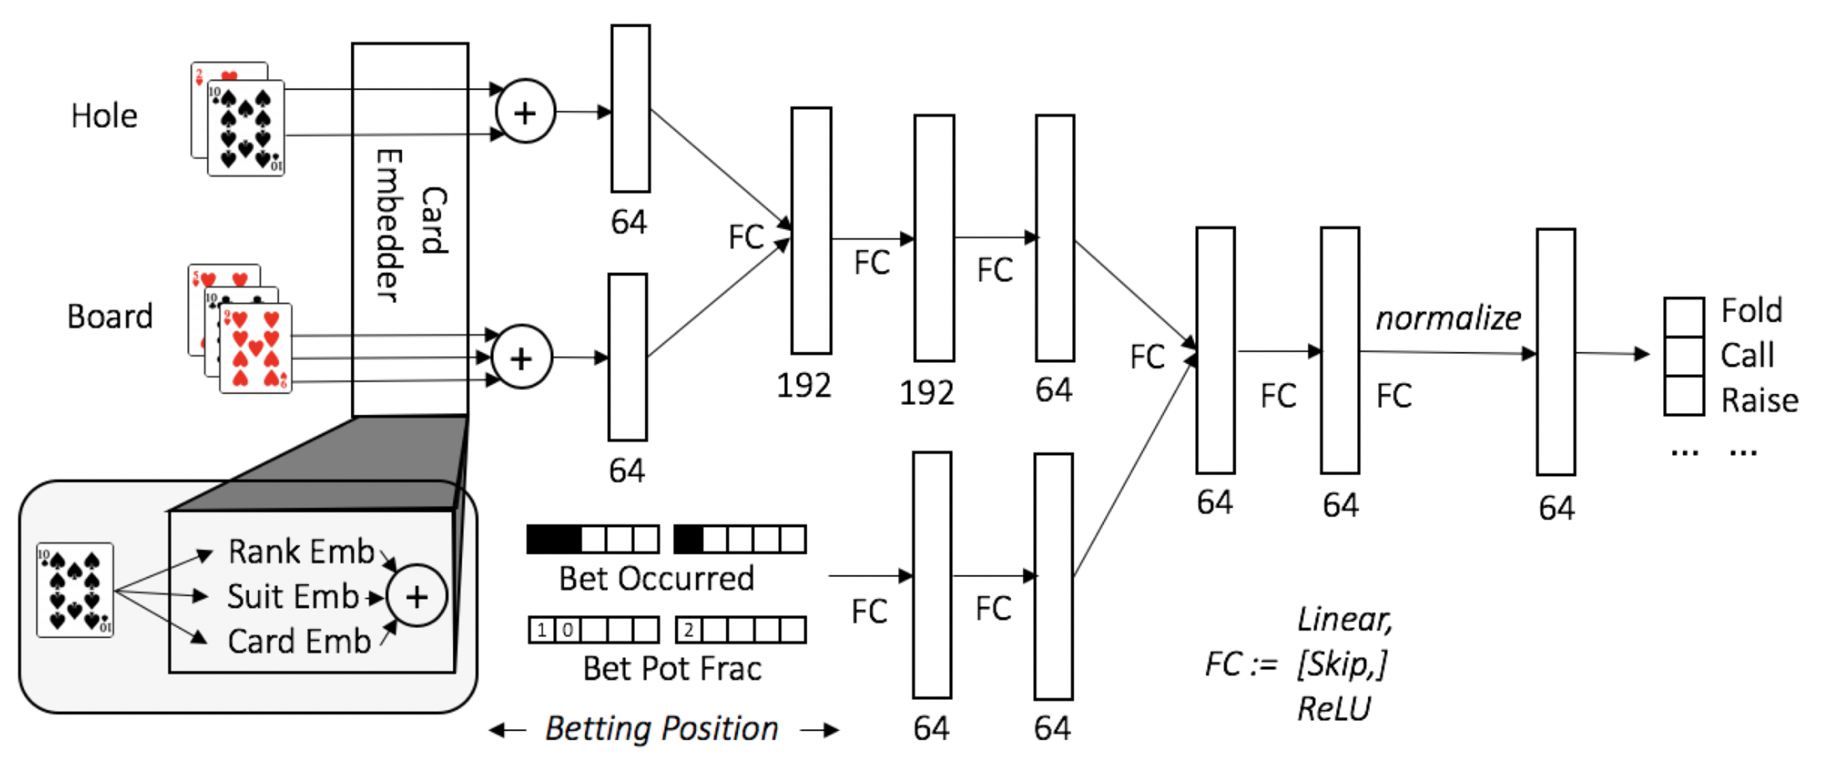
\includegraphics[width=\columnwidth]{nn_arch_FastModel.png}
\label{fig:nn_arch}
\vspace{-3mm}
\caption{\small{The neural network architecture used for Deep CFR. The network takes an infoset (observed cards and bet history) as input and outputs values (advantages or probability logits) for each possible action.}}
\end{figure}

\subsection{Model training}
\vspace{-0.03in}
We allocate a maximum size of 40 million infosets to each player's advantage memory $\mathcal{M}_{V,p}$  and the strategy memory $\mathcal{M}_{\Pi}$.
%Once a memory is full it is updated via reservoir sampling, maintaining a uniform distribution over infoset values from all prior iterations. We record the iteration at which each sample was collected to weight the training loss for linear CFR. 
The value model is trained from scratch each CFR iteration, starting from a random initialization. We perform 4,000 mini-batch stochastic gradient descent (SGD) iterations using a batch size of 10,000 and perform parameter updates using the Adam optimizer \cite{Kingma14:Adam} with a learning rate of $0.001$, with gradient norm clipping to $1$. For HULH we use 32,000 SGD iterations and a batch size of 20,000. Figure~\ref{fig:ablations} shows that training the model from scratch at each iteration, rather than using the weights from the previous iteration, leads to better convergence.

\subsection{Linear CFR}
\vspace{-0.03in}
There exist a number of variants of CFR that achieve much faster performance than vanilla CFR. However, most of these faster variants of CFR do not handle approximation error well~\cite{Tammelin15:Solving,Burch17:Time,Brown19:Solving,Schmid19:Variance}. In this paper we use \emph{Linear CFR (LCFR)}~\cite{Brown19:Solving}, a variant of CFR that is faster than CFR and in certain settings is the fastest-known variant of CFR (particularly in settings with wide distributions in payoffs), and which tolerates approximation error well. LCFR is not essential and does not appear to lead to better performance asymptotically, but does result in faster convergence in our experiments.

LCFR is like CFR except iteration $t$ is weighed by $t$. Specifically, we maintain a \emph{weight} on each entry stored in the advantage memory and the strategy memory, equal to $t$ when this entry was added. When training $\theta_p$ each iteration $T$, we rescale all the batch weights by $\frac{2}{T}$ and minimize weighted error.

% \adam{This needs to be fixed up. LCFR is a variant of DCFR. And we should write all the theory in terms of standard CFR.}. Formally, regret is defined as
% \begin{equation}
% R^T(I,a) = \sum_{t=1}^T\big(t r^t(I,a)\big)
% \label{eq:regret}
% \end{equation}
% and the average strategy is defined as
% \begin{equation}
% \bar{\sigma}_p^T(I) = \frac{\sum_{t = 1}^T \big(t\pi_p^{\sigma^t}(I)\sigma_p^t(I)\big)}{\sum_{t = 1}^T \big(t\pi_p^{\sigma^t}(I)\big)}
% \label{eq:average}
% \end{equation}
% We will use these definitions for regret and average strategy throughout the paper.
%Alternating updates with LCFR is in practice up to two orders of magnitude faster than vanilla CFR in large benchmark games.


\section{Experimental Results}
\vspace{-0.03in}
Figure~\ref{fig:abstraction} compares the performance of Deep CFR to different-sized domain-specific abstractions in FHP. The abstractions are solved using external-sampling Linear Monte Carlo CFR~\cite{Lanctot09:Monte,Brown19:Solving}, which is the leading algorithm in this setting. The 40,000 cluster abstraction means that the more than $10^9$ different decisions in the game were clustered into 40,000 abstract decisions, where situations in the same bucket are treated identically. This bucketing is done using K-means clustering on domain-specific features. The \emph{lossless abstraction} only clusters together situations that are strategically isomorphic (e.g., flushes that differ only by suit), so a solution to this abstraction maps to a solution in the full game without error.

Performance and exploitability are measured in terms of milli big blinds per game (mbb/g), which is a standard measure of win rate in poker.

The figure shows that Deep CFR asymptotically reaches a similar level of exploitability as the abstraction that uses 3.6 million clusters, but converges substantially faster. Although Deep CFR is more efficient in terms of nodes touched, neural network inference and training requires considerable overhead that tabular CFR avoids. However, Deep CFR does not require advanced domain knowledge. We show Deep CFR performance for 10,000 CFR traversals per step. Using more traversals per step is less sample efficient and requires greater neural network training time but requires fewer CFR steps.

Figure~\ref{fig:abstraction} also compares the performance of Deep CFR to NFSP, an existing method for learning approximate Nash equilibria in imperfect-information games. NFSP approximates fictitious self-play, which is proven to converge to a Nash equilibrium but in practice does so far slower than CFR. We observe that Deep CFR reaches an exploitability of 37 mbb/g while NFSP converges to 47 mbb/g.\footnote{We run NFSP with the same model architecture as we use for Deep CFR. In the benchmark game of Leduc Hold'em, our implementation of NFSP achieves an average exploitability (total exploitability divided by two) of 37 mbb/g in the benchmark game of Leduc Hold'em, which is substantially lower than originally reported in \citet{Heinrich16:Deep}. We report NFSP's best performance in FHP across a sweep of hyperparameters.} We also observe that Deep CFR is more sample efficient than NFSP. However, these methods spend most of their wallclock time performing SGD steps, so in our implementation we see a less dramatic improvement over NFSP in wallclock time than sample efficiency. 

Figure~\ref{fig:traversals} shows the performance of Deep CFR using different numbers of game traversals, network SGD steps, and model size. As the number of CFR traversals per iteration is reduced, convergence becomes slower but the model converges to the same final exploitability. This is presumably because it takes more iterations to collect enough data to reduce the variance sufficiently. On the other hand, reducing the number of SGD steps does not change the rate of convergence but affects the asymptotic exploitability of the model. This is presumably because the model loss decreases as the number of training steps is increased per iteration (see Theorem \ref{th:deepcfr_approx}). Increasing the model size also decreases final exploitability up to a certain model size in FHP. 

In Figure~\ref{fig:ablations} we consider ablations of certain components of Deep CFR. Retraining the regret model from scratch at each CFR iteration converges to a substantially lower exploitability than fine-tuning a single model across all iterations. We suspect that this is because a single model gets stuck in bad local minima as the objective is changed from iteration to iteration. The choice of reservoir sampling to update the memories is shown to be crucial; if a sliding window memory is used, the exploitability begins to increase once the memory is filled up, even if the memory is large enough to hold the samples from many CFR iterations.


Finally, we measure head-to-head performance in HULH. We compare Deep CFR and NFSP to the approximate solutions (solved via Linear Monte Carlo CFR) of three different-sized abstractions: one in which the more than $10^{14}$ decisions are clustered into $3.3 \cdot 10^6$ buckets, one in which there are $3.3 \cdot 10^7$ buckets and one in which there are $3.3 \cdot 10^8$ buckets. The results are presented in Table~\ref{tab:limit}. For comparison, the largest abstractions used by the poker AI Polaris in its 2007 HULH man-machine competition against human professionals contained roughly $3 \cdot 10^8$ buckets. When variance-reduction techniques were applied, the results showed that the professional human competitors lost to the 2007 Polaris AI by about $52 \pm 10$ mbb/g~\cite{Johanson16:Robust}. In contrast, our Deep CFR agent loses to a $3.3 \cdot 10^8$ bucket abstraction by only $-11 \pm 2$ mbb/g and beats NFSP by $43 \pm 2$ mbb/g.
%Our Deep CFR agent ties the abstraction-based strategy with a score of $3 \pm 12$ mbb/g.

% \begin{table}[h]
% \small
% \begin{center}
% \begin{tabular}{ l | c c c}
% \toprule
%               & \multicolumn{3}{c}{\bf Opponent Abstraction Size} \\
% {\bf Model}    & $3.3 \cdot 10^6$ & $3.3 \cdot 10^7$ & $3.3 \cdot 10^8$ \\
% \midrule
% NFSP           &$ -40 \pm 2 $ mbb/g&$ -49 \pm 2 $ mbb/g&$ -55 \pm 2 $ mbb/g \\
% Deep CFR       &$ \ +6 \pm 2 $ mbb/g&$ \ -6 \pm 2 $ mbb/g&$ -11 \pm 2 $ mbb/g \\
% \bottomrule
% \end{tabular}
% \end{center}
% \vspace{-3mm}
% \caption{Head-to-head expected value of NFSP and Deep CFR in HULH against converged CFR equilibria with varying abstraction sizes. For comparison, in 2007 an AI using abstractions of roughly $3 \cdot 10^8$ buckets defeated human professionals by about $52$ mbb/g after variance reduction techniques were applied. Deep CFR has an expected value of $+43 \pm 2$ mbb/g against NFSP.
% %\adam{Mention something about the 300M abstraction being professional level?}
% }
% \label{tab:limit}
% \end{table}



\begin{table*}[t]
\small
\begin{center}
\begin{tabular}{ l | c c | c c c}
\toprule
               & \multicolumn{4}{c}{\bf Opponent Model} & \\
               &      & \multicolumn{1}{ c}{} & \multicolumn{3}{| c }{ Abstraction Size} \\
{\bf Model}    & NFSP & Deep CFR & \multicolumn{1}{| c}{ $3.3 \cdot 10^6$} & $3.3 \cdot 10^7$ & $3.3 \cdot 10^8$ \\
\midrule
NFSP           & - & $-43 \pm 2$ mbb/g &$ -40 \pm 2 $ mbb/g&$ -49 \pm 2 $ mbb/g&$ -55 \pm 2 $ mbb/g \\
Deep CFR       & $+43 \pm 2$ mbb/g & - &$ \ +6 \pm 2 $ mbb/g&$ \ -6 \pm 2 $ mbb/g&$ -11 \pm 2 $ mbb/g \\
\bottomrule
\end{tabular}
\end{center}
\vspace{-3mm}
\caption{Head-to-head expected value of NFSP and Deep CFR in HULH against converged CFR equilibria with varying abstraction sizes. For comparison, in 2007 an AI using abstractions of roughly $3 \cdot 10^8$ buckets defeated human professionals by about $52$ mbb/g (after variance reduction techniques were applied).
%\adam{Mention something about the 300M abstraction being professional level?}
}
\label{tab:limit}
\end{table*}

%\vspace{-0.1in}
%\vspace{-0.15in}
\begin{figure}[h!]
\centering
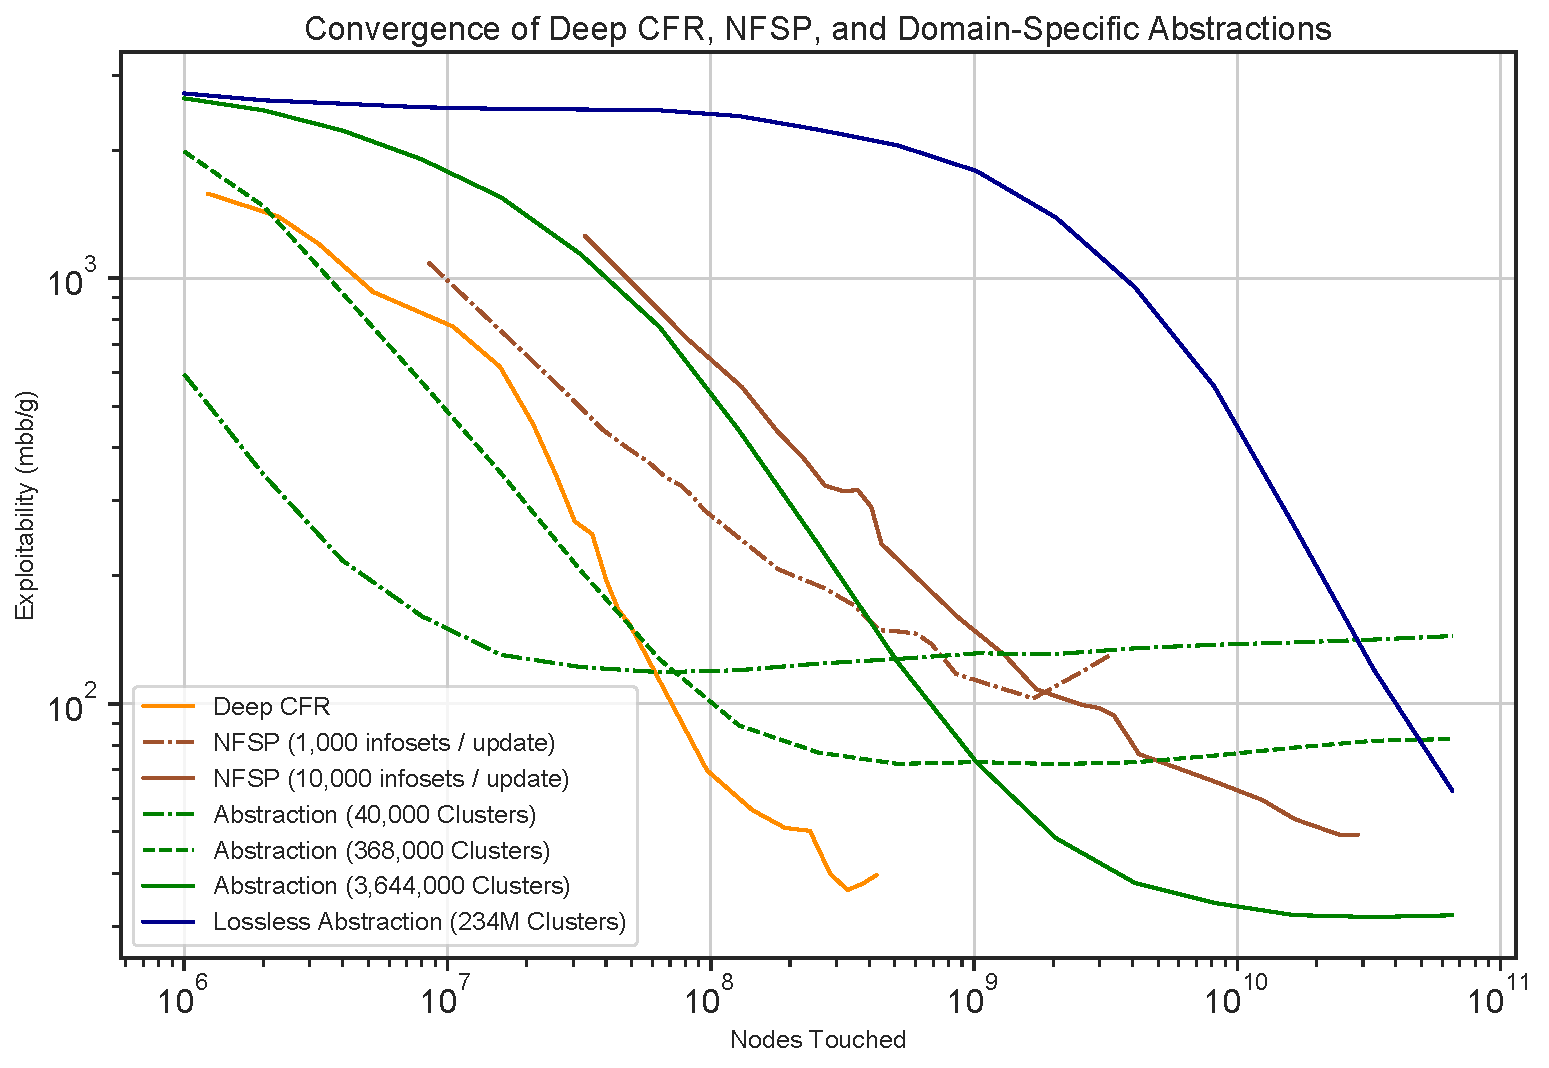
\includegraphics[width=3.3in]{cfr_v_tab.pdf}
\vspace{-3mm}
\caption{\small{Comparison of Deep CFR with domain-specific tabular abstractions and NFSP in FHP. Coarser abstractions converge faster but are more exploitable. Deep CFR converges with 2-3 orders of magnitude fewer samples than a lossless abstraction, and performs competitively with a 3.6 million cluster abstraction. Deep CFR achieves lower exploitability than NFSP, while traversing fewer infosets.}}
\label{fig:abstraction}
\end{figure}

\begin{figure*}[h]
\centering
\hspace{-.5cm}
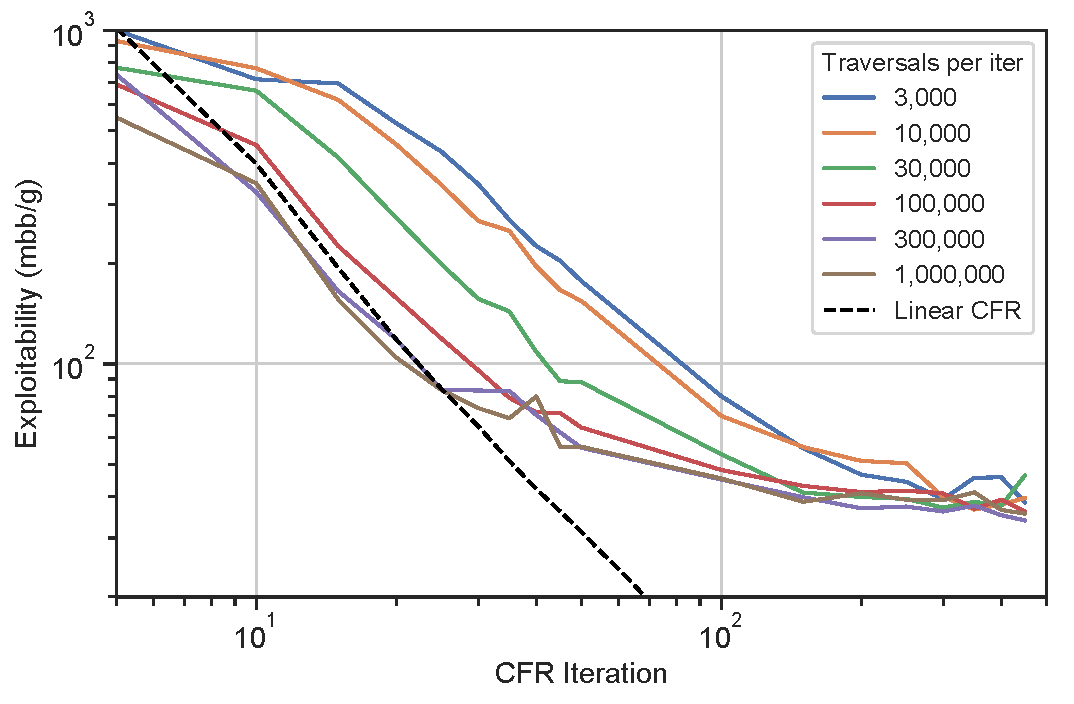
\includegraphics[width=2.3in]{traversals.pdf}
\hspace{-.2cm}
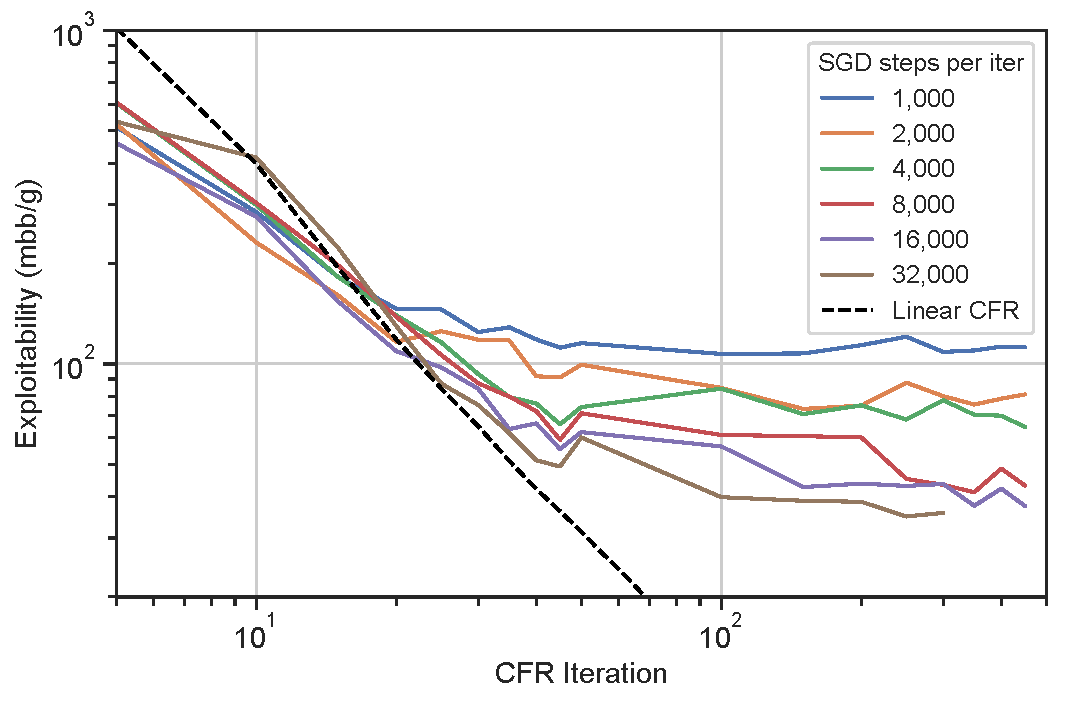
\includegraphics[width=2.3in]{cfr_training.pdf}
\hspace{-.2cm}
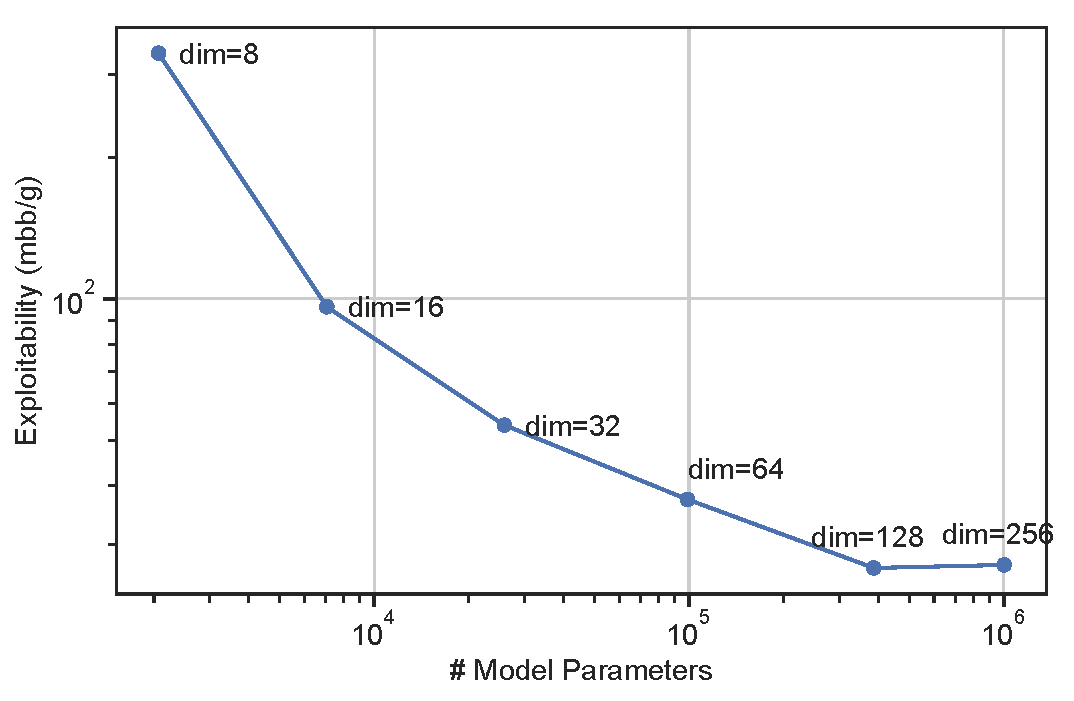
\includegraphics[width=2.3in]{dim.pdf}

\vspace{-3mm}
\caption{\small{\textbf{Left:} FHP convergence for different numbers of training data collection traversals per simulated LCFR iteration. The dotted line shows the performance of vanilla tabular Linear CFR without abstraction or sampling. \textbf{Middle:} FHP convergence using different numbers of minibatch SGD updates to train the advantage model at each LCFR iteration. \textbf{Right:} Exploitability of Deep CFR in FHP for different model sizes. Label indicates the dimension (number of features) in each hidden layer of the model.}}
\label{fig:traversals}
\end{figure*}

% \begin{figure}[h!]
% 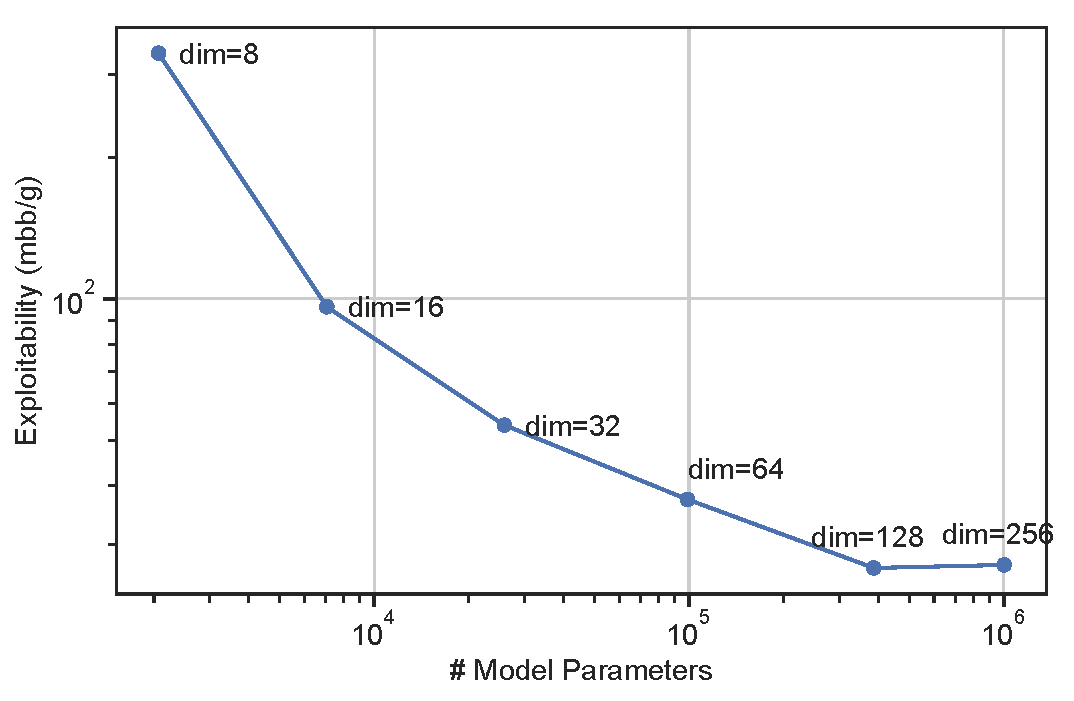
\includegraphics[width=3.2in]{dim.pdf}
% \vspace{-3mm}
% \caption{\small{}}
% \label{fig:dim}
% \end{figure}

\begin{figure*}[h!]
\hspace{1cm}
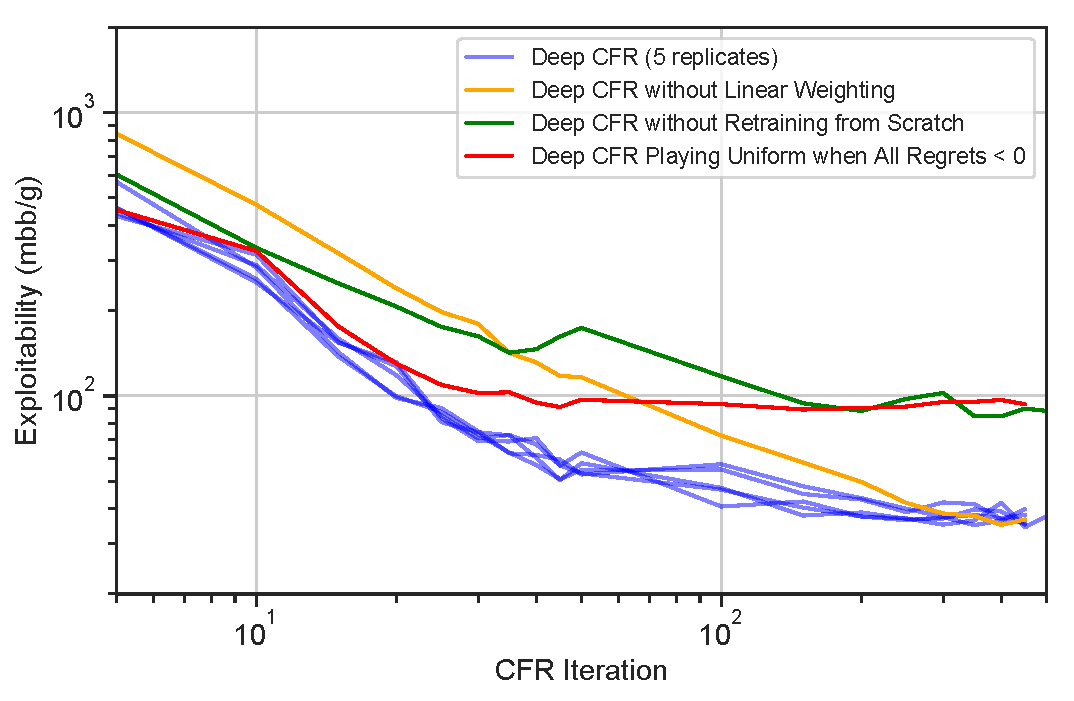
\includegraphics[width=2.5in]{ablations_replicates.pdf}
\hspace{.5cm}
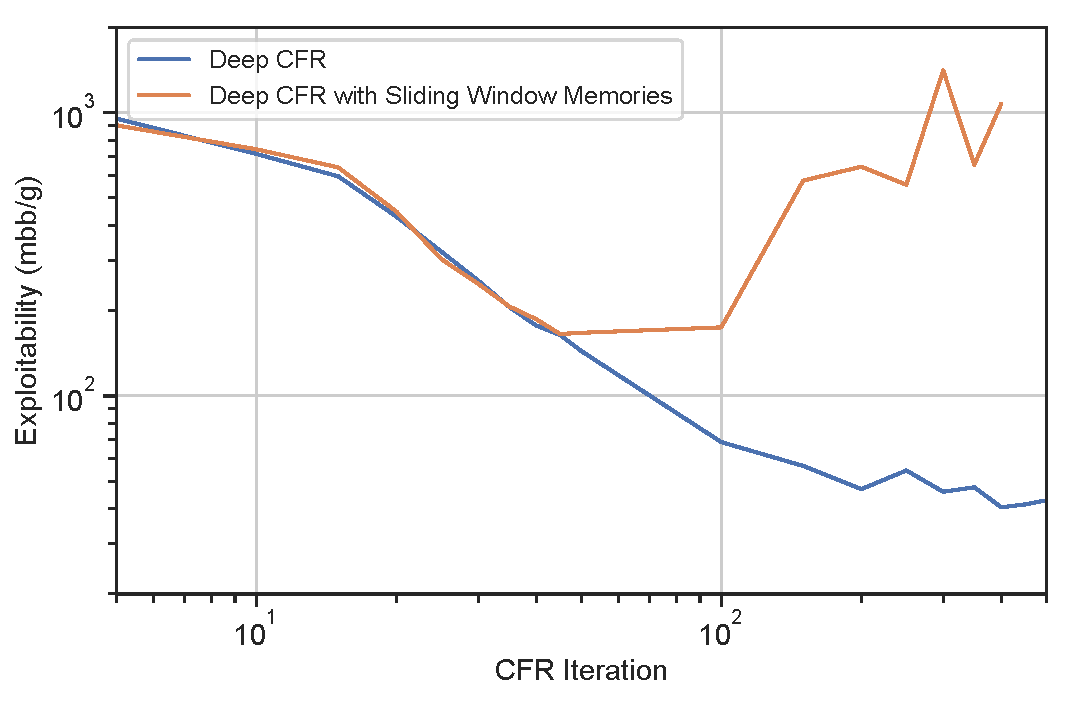
\includegraphics[width=2.5in]{reservoir.pdf}
\vspace{-3mm}
\caption{\small{Ablations of Deep CFR components in FHP. \textbf{Left:} As a baseline, we plot 5 replicates of Deep CFR, which show consistent exploitability curves (standard deviation at $t=450$ is $2.25$ mbb/g). Deep CFR without linear weighting converges to a similar exploitability, but more slowly. If the same network is fine-tuned at each CFR iteration rather than training from scratch, the final exploitability is about 50\% higher. Also, if the algorithm plays a uniform strategy when all regrets are negative (i.e. standard regret matching), rather than the highest-regret action, the final exploitability is also 50\% higher. \textbf{Right:} If Deep CFR is performed using sliding-window memories, exploitability stops converging once the buffer becomes full\footnote{With our standard hyperparameters, the memory fills up in just 1-2 iterations, so for this experiment we perform only 10,000 CFR traversals per iteration to demonstrate that convergence ceases once the buffer fills up after about 50 iterations.}. However, with reservoir sampling, convergence continues after the memories are full.}}
\label{fig:ablations}
\end{figure*}



% \begin{table*}[h]
% \small
% \begin{center}
% \begin{tabular}{ l | c c c c}
% \toprule
%               & \multicolumn{3}{c}{\bf Opponent Abstraction Size} & \multicolumn{1}{|c}{}  \\
% {\bf Model}    & $3.3 \cdot 10^6$ & $3.3 \cdot 10^7$ & $3.3 \cdot 10^8$ & \multicolumn{1}{|c}{NFSP}  \\
% \midrule
% NFSP           &$ -40 \pm 2 $ mbb/g&$ -49 \pm 2 $ mbb/g&$ -55 \pm 2 $ mbb/g & - \\
% Deep CFR       &$ \ +6 \pm 2 $ mbb/g&$ \ -6 \pm 2 $ mbb/g&$ -11 \pm 2 $ mbb/g & $+43 \pm 2$ mbb/g \\
% \bottomrule
% \end{tabular}
% \end{center}
% \vspace{-3mm}
% \caption{Head-to-head expected value of NFSP and Deep CFR in HULH against converged CFR equilibria with varying abstraction sizes. For comparison, in 2007 an AI using abstractions of roughly $3 \cdot 10^8$ buckets defeated human professionals by about $52$ mbb/g after variance reduction techniques were applied.
% %\adam{Mention something about the 300M abstraction being professional level?}
% }
% \label{tab:limit}
% \end{table*}


% \begin{table}[h]
% \small
% \begin{center}
% \begin{tabular}{ l  | r }
% \toprule
% \bf Opponent Model & \bf Expected Payoff \\
% \midrule
% NFSP  & $43 \pm 2$ mbb/g \\
% $3.3 \cdot 10^6$ Cluster Abstraction & $6 \pm 2$ mbb/g \\
% $3.3 \cdot 10^6$ Cluster Abstraction & $-6 \pm 2$ mbb/g \\
% $3.3 \cdot 10^6$ Cluster Abstraction & $-11 \pm 2$ mbb/g \\
% \bottomrule
% \end{tabular}
% \end{center}
% \vspace{-3mm}
% \caption{\adam{FIXME: Delete this table or the one above}}
% \label{tab:limit}
% \end{table}

\section{Conclusions}
\vspace{-0.03in}
%We introduced a deep neural network implementation of CFR that is theoretically principled and achieves performance comparable to domain-specific abstraction techniques in flop hold'em poker while not relying on advanced domain knowledge. This is the first successful application of deep learning to CFR in a large game. As a next step, we hope to improve and scale the techniques presented in this paper to produce a competitive AI in the benchmark game of heads-up no-limit Texas hold'em.

We describe a method to find approximate equilibria in large imperfect-information games by combining the CFR algorithm with deep neural network function approximation. This method is theoretically principled and achieves strong performance in large poker games relative to domain-specific abstraction techniques without relying on advanced domain knowledge. This is the first non-tabular variant of CFR to be successful in large games.

Deep CFR and other neural methods for imperfect-information games provide a promising direction for tackling large games
%such as StarCraft$^{\tiny \textregistered}$, Stratego$^{\tiny \textregistered}$, or 9-player poker,
whose state or action spaces are too large for tabular methods and where abstraction is not straightforward. Extending Deep CFR to
%these
larger games will likely require more scalable sampling strategies than those used in this work, as well as strategies to reduce the high variance in sampled payoffs. Recent work has suggested promising directions both for more scalable sampling \cite{Li18:Double} and variance reduction techniques \cite{Schmid19:Variance}. We believe these are important areas for future work.

\clearpage


\bibliography{dairefs}
\bibliographystyle{icml2019}

\clearpage

\newpage

\appendix

\onecolumn

\section{Rules for Heads-Up Limit Texas Hold'em and Flop Hold'em Poker}
\label{sec:rules}
Heads-up limit Texas hold'em is a two-player zero-sum game. There are two players and the position of the two players alternate after each hand. On each betting round, each player can choose to either fold, call, or raise. Folding results in the player losing and the money in the pot being awarded to the other player. Calling means the player places a number of chips in the pot equal to the opponent's share. Raising means that player adds more chips to the pot than the opponent's share. A round ends when a player calls (if both players have acted). There cannot be more than three raises in the first or second betting round or more than four raises in the third or fourth betting round, so there is a limited number of actions in the game. Raises in the first two rounds are \$100 and raises in the second two rounds are \$200.

At the start of each hand of HULH, both players are dealt two private cards from a standard 52-card deck. $P_1$ must place \$50 in the pot and $P_2$ must place \$100 in the pot. A round of betting then occurs starting with $P_1$. When the round ends, three \emph{community} cards are dealt face up that both players can ultimately use in their final hands. Another round of betting occurs, starting with $P_2$ this time. Afterward another community card is dealt face up and another betting round occurs. Then a final card is dealt face up and a final betting round occurs. At the end of the betting round, unless a player has folded, the player with the best five-card poker hand constructed from their two private cards and the five community cards wins the pot. In the case of a tie, the pot is split evenly.

Flop Hold'em Poker is identical to HULH except there are only the first two betting rounds.

% \section{Proof of Theorem~\ref{th:deepcfr}}
% \begin{proof}
% Consider an information set $I$ in which player~$p$ acts. Let $\tilde{v}^{\sigma^t}(I,a)$ be the expected value return by the external sampling iteration for infoset $I$ action $a$ and let $\tilde{v}^{\sigma^t}(I,a)$ be the value for infoset $I$. From Lemma~1 in \cite{Lanctot09:Monte}, we know that $E[\tilde{v}^{\sigma^t}(I)] = v^{\sigma^t}(I)$ and $E[\tilde{v}^{\sigma^t}(I,a)] = v^{\sigma^t}(I,a)$. Since $K \rightarrow \infty$, so the average of all samples $\tilde{d}^{\sigma^t}(I,a) = \tilde{v}^{\sigma^t}(I,a) - \tilde{v}^{\sigma^t}(I)$ in the memory approaches $E[\tilde{v}^{\sigma^t}(I,a) - \tilde{v}^{\sigma^t}(I)] = v^{\sigma^t}(I,a) - v^{\sigma^t}(I) = d^{\sigma^t}(I,a)$.

% Let $n_t$ be the number of samples of $I$ on iteration $t$. The probability that $I$ is sampled during a traversal on iteration $t$ is $\pi^{\sigma^t}_{-p}(I)$. Since there are $K$ traversals on each iteration, so $E[n_t] = K \pi^{\sigma^t}_{-p}(I)$ and $E[\frac{t n_t}{\sum_{t'=1}^T (t n_{t'})}] = \frac{t \pi^{\sigma^t}_{-p}(I)}{\sum_{t'=1}^T \big(t \pi^{\sigma^{t'}}_{-p}(I)\big)}$. Since $K \rightarrow \infty$, so $\frac{t n_t}{\sum_{t'=1}^T (t n_{t'})} \rightarrow E[\frac{t n_t}{\sum_{t'=1}^T (t n_{t'})}] = \frac{t \pi^{\sigma^t}_{-p}(I)}{\sum_{t'=1}^T \big(t \pi^{\sigma^{t'}}_{-p}(I)\big)}$.

% Since samples from iteration $t$ are assigned weight $t$ and since the value network achieves minimum error, so $\hat{D}^T(I,a) = \frac{\sum_{t=1}^T \big(t \pi_{-p}^{\sigma^t}(I) d^{\sigma^t}(I,a)\big)}{\sum_{t=1}^T \big(t \pi_{-p}^{\sigma^{t}}(I)\big)} = D^T(I,a)$.

% Similarly, since samples from iteration $t$ are assigned weight $t$ and since the policy network achieves minimum error, so $\hat{\sigma}^T(I,a) = \frac{\sum_{t=1}^T \big(t \pi_{-p}^{\sigma^t}(I) \sigma^t(I,a)\big)}{\sum_{t=1}^T \big(t \pi_{-p}^{\sigma^{t}}(I)\big)} = \bar{\sigma}^T(I,a)$.

% We present the proof assuming Deep CFR is using vanilla CFR. All other forms of CFR easily follow.
% Define $\hat{R}^t(I,a) = \hat{D}^t(I,a) \sum_{t'=1}^t \pi_{-P(I)}^{\sigma^{t'}}(I)$.
% Since $|\hat{D}^t(I,a) - D^t(I,a)| \le \epsilon \big( \frac{t}{\sum_{t' = 1}^t \pi^{\sigma^{t'}}_{-P(I)}}\big)$, so $|\hat{R}^t(I,a) - R^t(I,a)| \le \epsilon t$. 

% From Theorem~3.0.7 in \cite{Morrill16:Using}, we know that if $\sum_{a \in A(I)} |\hat{R}^t(I,a) - R^t(I,a)| \le t \epsilon$ for every infoset $I$ in which $p \in \mathcal{P}$ acts, then external regret for $p$ is bounded by $\sum_{I \in \mathcal{I}_p} \Delta \sqrt{|A(I)|} \sqrt{ \big(T + \frac{4 \Delta \sum_{t = 1}^T (t \epsilon)}{\sqrt{|A(I)|}} \big)}$. Since $\sum_{t = 1}^T t = \frac{T(T+1)}{2}$ we get that external regret for $p$ is bounded by $\sum_{I \in \mathcal{I}_p} \Delta \sqrt{|A(I)|} \sqrt{T} \sqrt{ \big(1 + \frac{2 \Delta (T + 1) \epsilon}{\sqrt{|A(I)|}} \big)}$

% \begin{theorem}
% Assume on each iteration $t$ that $|\hat{D}^t(I,a) - D^t(I,a)| \le \frac{t \epsilon}{\sum_{t' = 1}^t \pi^{\sigma^{t'}}_{-P(I)}}$. After $T$ iterations of Deep CFR, external regret for player $p$ is bounded by $\delta_p = \Big(\sum_{I \in \mathcal{I}_p} \Delta \sqrt{|A(I)|} \sqrt{ \big(T + \frac{2 \epsilon T^2}{\Delta\sqrt{|A(I)|}}\big)}\Big)$.
% \label{th:deepcfr}
% \end{theorem}

% \begin{corollary}
% Assume on each iteration $t$ that $|\hat{D}^t(I,a) - D^t(I,a)| \le \frac{t\epsilon}{\sum_{t' = 1}^t \pi^{\sigma^{t'}}_{-P(I)}}$. After $T$ iterations of Deep CFR in a two-player zero-sum game the average strategies form a $(\delta_1 + \delta_2)$-Nash equilibrium.
% \label{th:deepnash}
% \end{corollary}


%\end{proof}

% \section{Proof of Lemma \ref{lemma:mc_regret_ev}}

% In external sampling MCCFR, in each block $Q_j$ the player's actions are all traversed while opponent and chance actions are sampled. For ES MCCFR, the reweighting factor $q(z)=\pi_{-p}^\sigma(z)$ (\citealt{lanctot2013monte}, Sec. 4.3).

% \begin{align}
% \mathbb{E}_{Q\in \mathcal{Q}}\left[ \tilde{v}_p(I,a) | I \in Q \right] & = \mathbb{E}_{\sigma^{-p}}\left[ \right]
% \end{align}

\section{Proofs of Theorems}
\label{app:proof}
\subsection{Review of MCCFR}

We begin by reviewing the derivation of convergence bounds for external sampling MCCFR from \citealt{Lanctot09:Monte}.

An MCCFR scheme is completely specified by a set of \emph{blocks} $\mathcal{Q}=\{Q_i\}$ which each comprise a subset of all terminal histories $Z$. On each iteration MCCFR samples one of these blocks, and only considers terminal histories within that block. Let $q_j > 0$ be the probability of considering block $Q_j$ in an iteration. 

Let $Z_I$ be the set of terminal nodes that contain a prefix in $I$, and let $z[I]$ be that prefix. 
Define $\pi^\sigma(h\to z)$ as the probability of playing to $z$ given that player $p$ is at node $h$ with both players playing $\sigma$. $$\pi^\sigma(h\to z) = \sum_{z\in Z_I} \frac{\pi^\sigma(z[I])}{\pi^\sigma(I)}  \pi^\sigma(z).$$ 
$\pi^\sigma(I\to z)$ is undefined when $\pi(I)=0$.

Let $q(z)=\sum_{j:z\in Q_j}{q_j}$ be the probability that terminal history $z$ is sampled in an iteration of MCCFR. For external sampling MCCFR, $q(z)=\pi^\sigma_{-i}(z)$.

The \emph{sampled value} $\tilde{v}^\sigma_i(I|j)$ when sampling block $j$ is

\begin{equation}
    \tilde{v}_p^\sigma(I|j) = \sum_{z\in Q_j \cap Z_I}{
        \frac{1}{q(z)}
        u_p(z)
        \pi^\sigma_{-p}(z[I])
        \pi^\sigma(z[I] \to z)
    }
\end{equation}

For external sampling, the sampled value reduces to
\begin{equation}
        \tilde{v}^\sigma_p(I|j) = \sum_{z\in Q_j \cap Z_I}{
        u_p(z)
        \pi_p^\sigma(z[I] \to z)
    }
\end{equation}

The sampled value is an unbiased estimator of the true value $v_p(I)$. Therefore the \textit{sampled instantaneous regret} $\tilde{r}^t(I,a) = \tilde{v}_p^{\sigma^t}(I,a) - \tilde{v}_p^{\sigma^t}(I)$ is an unbiased estimator of $r^t(I,a)$.

The \textit{sampled regret} is calculated as $\tilde{R}^T(I,a)=\sum_{t=1}^T \tilde{r}^t(I,a)$.

We first state the general bound shown in \cite{lanctot2013monte}, Theorem 3.

\citealt{lanctot2013monte} defines $\mathcal{B}_p$ to be a set with one element per distinct action sequence $\vec{a}$ played by $p$, containing all infosets that may arise when $p$ plays $\vec{a}$. $M_p$ is then defined by $\sum_{B \in \mathcal{B}_p} |B|$.   Let $\Delta$ be the difference between the maximum and minimum payoffs in the game.

\begin{theorem} (\citealt{lanctot2013monte}, Theorem 3)
For any $p \in (0,1]$, when using any algorithm in the MCCFR family such that for all $Q\in \mathcal{Q}$ and B $\in \mathcal{B}_p$,
\begin{equation}
    \sum_{I\in B}\left( 
        \sum_{z \in Q \cap Z_I}{
            \frac{
                \pi^\sigma(z[I] \to z)\pi^\sigma_{-p}(z[I])
            }{
                q(z)
            }
        }
    \right)^2 \leq \frac{1}{\delta^2}
\label{thm:lanctot_general_cond}
\end{equation}

where $\delta \leq 1$, then with probability at least $1-\rho$, total regret is bounded by

\begin{equation}
    R_p^T \leq
    \left( M_p + \frac{\sqrt{2|\mathcal{I}_p||\mathcal{B}_p|}}{\sqrt{\rho}} \right)
    \left( \frac{1}{\delta} \right)
    \Delta \sqrt{|A|T}
\label{thm:lanctot_general}
\end{equation}
.
\end{theorem}

For the case of external sampling MCCFR, $q(z)=\pi^\sigma_{-i}(z)$. \citealt{Lanctot09:Monte}, Theorem 9 shows that for external sampling, for which $q(z)=\pi^\sigma_{-i}(z)$, the inequality in (\ref{thm:lanctot_general_cond}) holds for $\delta=1$, and thus the bound implied by (\ref{thm:lanctot_general}) is

\begin{align}
    \bar{R}_p^T \leq &
    \left( M_p + \frac{\sqrt{2|\mathcal{I}_p||\mathcal{B}_p|}}{\sqrt{\rho}} \right)
    \Delta \frac{\sqrt{|A|}}{\sqrt{T}} \\
    \leq & \left(1 + \frac{\sqrt{2}}{\sqrt{\rho K}}\right)\Delta |\mathcal{I}_p| \frac{\sqrt{|A|}}{\sqrt{T}} \hspace{2cm} \textrm{because $|\mathcal{B}_p| \leq M_p \leq |\mathcal{I}_p|$}
\label{thm:lanctot_external1}
\end{align}
.

\subsection{Proof of Lemma \ref{lemma:value_lemma}}
\label{app:value_lemma}

We show $$\mathbb{E}_{Q_j\sim \mathcal{Q}} \left[ \tilde{v}_p^{\sigma^t}(I) \middle|  Z_I \cap Q_j \neq \emptyset \right] = v^{\sigma^t}(I) / \pi_{-p}^{\sigma^t}(I).$$

Let $q_j = P(Q_j)$.
\begin{align*}
    \mathbb{E}_{Q_j\sim \mathcal{Q}} \left[ \tilde{v}_p^{\sigma^t}(I) \middle| Z_I \cap Q \neq \emptyset \right] & = \frac{\mathbb{E}_{Q_j\sim \mathcal{Q}} \left[ \tilde{v}_p^{\sigma^t}(I) \right] }{ P_{Q_j \sim \mathcal{Q}}(Z_I \cap Q_j \neq \emptyset)} \\
    & = \frac{\sum_{Q_j\in \mathcal{Q}} q_j \sum_{z\in Z_I \cap Q_j} u_p(z) \pi_{-p}^{\sigma^t}(z[I]) \pi^{\sigma^t}(z[I] \to z) / q(z) }{ \pi_{-p}^{\sigma^t}(I)} \\
    & = \frac{  \sum_{z\in Z_I \cap Q_j} \left( \sum_{Q_j: z \in Q_j} q_j \right) u_p(z) \pi_{-p}^{\sigma^t}(z[I]) \pi^{\sigma^t}(z[I] \to z) / q(z) }{ \pi_{-p}^{\sigma^t}(I)} \\
    & = \frac{ \sum_{z\in Z_I} q(z) u_p(z) \pi_{-p}^{\sigma^t}(z[I]) \pi^{\sigma^t}(z[I] \to z) / q(z) }{ \pi_{-p}^{\sigma^t}(I)} \hspace{1cm} \textrm{By definition of $q(z)$} \\
    & = \frac{ v^{\sigma^t}(I) }{\pi_{-p}^{\sigma^t}(I)}
\end{align*}

%  \\
%     & = \sum_{Q_j\in \mathcal{Q}_t} \sum_{z\in Z_I \cap Q_j} q_j \frac{ u_p(z) \pi^{\sigma^t}(I \to z) }{ \pi_{-p}^{\sigma^t}(I) \pi_{-p}^{\sigma^t}(z)} \\
%     & = \sum_{z\in Z_I} \left(\sum_{Q_j\in \mathcal{Q}_I }  q_j \right) \frac{ u_p(z) \pi^{\sigma^t}(I \to z) }{ \pi_{-p}^{\sigma^t}(I) \pi_{-p}^{\sigma^t}(z)} \hspace{1cm} \textrm{ where } \mathcal{Q}_{I} = \{Q : Q \in \mathcal{Q}_t \wedge Z_I \subseteq Q\} \\
%     & = \sum_{z\in Z_I} \pi_{-p}^{\sigma^t}(I) \frac{ u_p(z) \pi^{\sigma^t}(I \to z) }{ \pi_{-p}^{\sigma^t}(I) \pi_{-p}^{\sigma^t}(z)} \\
%     & = \sum_{z\in Z_I} \frac{ u_p(z) \pi^{\sigma^t}(I \to z) }{ \pi_{-p}^{\sigma^t}(I) } \\
%     & = v_p(I) / \pi_{-p}^{\sigma^t}(I)  \\
The result now follows directly.

\subsection{$K$-external sampling}

\newcommand{\Rp}[1]{R_{#1}^+(a)}
\newcommand{\Rsum}[1]{\Rp{{\Sigma,#1}}}
\newcommand{\aA}{\sum_{a\in A}}

We first show that performing MCCFR with $K$ external sampling traversals per iteration ($K$-ES) shares a similar convergence bound with standard external sampling (i.e. $1$-ES). We will refer to this result in the next section when we consider the full Deep CFR algorithm. This convergence bound is rather obvious and the derivation pedantic, so the reader is welcome to skip this section.

We model $T$ rounds of $K$-external sampling as $T\times K$ rounds of external sampling, where at each round $t \cdot K + d$ (for integer $t \geq 0$ and integer $0 \leq d < K$) we play

\begin{align}
\label{eq:rm2}
\sigma_{tK+d}(a) = 
\begin{cases}
\frac{\Rp{tK}}{R_{\Sigma,{tK}}^+}\textrm{\ if\ } R_{\Sigma,{tK}}^+ > 0 \\
\textrm{\ arbitrary,\ otherwise}
\end{cases}
\end{align}

In prior work, $\sigma$ is typically defined to play $\frac{1}{|A|}$ when $\Rsum{T} \leq 0$, but in fact the convergence bounds do not constraint $\sigma$'s play in these situations, which we will demonstrate explicitly here. We need this fact because minimizing the loss $\mathcal{L}(V)$ is defined only over the samples of (visited) infosets and thus does not constrain the strategy in unvisited infosets.

\begin{lemma}
\label{lemma:rmneg}
If regret matching is used in $K$-ES, then for $0 \leq d < K$
\begin{equation}
    \sum_{a\in A} \Rp{tK} r_{tK+d}(a) \leq 0
\end{equation}
\end{lemma}

\begin{proof}
If $R_{\Sigma,{tK}}^+ \leq 0$, then $R_{tK}^+(a)=0$ for all $a$ and the result follows directly. For $R_{\Sigma,{tK}}^+ > 0$,

\begin{align}
    \aA R_{tK}^+(a) r_{tK+d}(a) & = \aA R_T^+(a)(u_{tK+d}(a)-u_{tK+d}(\sigma_{tK})) \\
    & = \left( \aA R_{tK}^+(a) u_{tK+d}(a) \right) - 
         \left( u_{tK+d}(\sigma_{tK})\aA R_{tK}^+(a) \right) \\
    & = \left( \aA R_{tK}^+(a) u_{tK+d}(a) \right) - 
         \left( \aA \sigma_{tK+d}(a)u_{tK+d}(a) \right) \Rsum{tK} \\
    & = \left( \aA R_{tK}^+(a) u_{tK+d}(a) \right) - 
         \left( \aA \frac{\Rp{tK}}{\Rsum{tK}} u_{tK+d}(a) \right) \Rsum{tK} \\
    & = \left( \aA R_{tK}^+(a) u_{tK+d}(a) \right) - 
         \left( \aA \Rp{tK}(a) u_{tK+d}(a) \right) \\
    & = 0
\end{align}
\end{proof} 
% The proof of \citealt{Lanctot09:Monte}, Lemma 8 applies directly. \citealt{Lanctot09:Monte} only considers strategies that play $\frac{1}{|A|}$ when $R_{\Sigma,{tK}}^+ = 0$, but if $R_{\Sigma,{tK}}^+ = 0$, but the proof admits arbitrary strategies in this situation because if $R_{\Sigma,{tK}}^+ = 0$ then $R_T^+(a)=0$ for all $a$ and the result follows immediately.

\begin{theorem}
\label{th:blackwell}
Playing according to Equation \ref{eq:rm2} guarantees the following bound on total regret
\begin{equation}
    \sum_{a\in A}(\Rp{TK})^2 \leq |A|\Delta^2 K^2 T
\end{equation}
\end{theorem}

\begin{proof}

We prove by recursion on $T$.
\begin{align}
    \sum_{a\in A}(\Rp{TK})^2 \leq & 
    \sum_{a\in A}\left(\Rp{(T-1)K} + \sum_{d=0}^{K-1}{r_{tK-d}(a)} \right)^2 \\
    = & \sum_{a\in A} \biggl( R_{(T-1)K}^+(a)^2 +
        2 \sum_{d=0}^{K-1}r_d(a) R_{(T-1)K}^+(a) + \sum_{d=0}^{K-1}\sum_{d'=0}^{K-1}r_{TK-d}(a) r_{TK-d'}(a) \biggr)
\end{align}

By Lemma \ref{lemma:rmneg}, 

\begin{equation}
    \sum_{a\in A}(R_{TK}^+(a))^2 \leq 
            \sum_{a\in A} (R_{(T-1)K}^+(a))^2 +
            \sum_{a\in A} \sum_{d=0}^{K-1}\sum_{d'=0}^{K-1}r_{TK-d}(a) r_{TK-d'}(a)
\end{equation}

By induction,
\begin{equation}
    \sum_{a\in A}(R_{(T-1)K}^+(a))^2 \leq |A|\Delta^2 (T-1)
\end{equation}

From the definition, $|r_{TK-d}(a)|\leq \Delta$

\begin{align}
    \sum_{a\in A}(R_{TK}^+(a))^2 \leq 
           |A|\Delta^2 (T-1) + K^2 |A| \Delta^2
            = |A| \Delta^2 K^2 T 
\end{align}

\end{proof}

% \begin{corollary}
% \label{cor:blackwell}
% Average regret 

% \begin{equation}
%     (\bar{R}_{TK}^+(a))^2 = \left(\frac{R_{TK}^+(a)}{KT}\right)^2 \leq \frac{|A|\Delta^2}{T}
% \end{equation}
% \end{corollary}

\begin{theorem} (\citealt{lanctot2013monte}, Theorem 3 \& Theorem 5)
\label{thm:mccfr_bound}
After $T$ iterations of $K$-ES, average regret is bounded by

\begin{equation}
    \bar{R}_p^{TK} \leq
    \left( 1 + \frac{\sqrt{2}}{\sqrt{\rho K}} \right)
    |\mathcal{I}_p|\Delta \frac{\sqrt{|A|}}{\sqrt{T}}
\label{thm:lanctot_external2}
\end{equation}

% \begin{equation}
%     \bar{R}_p^{TK} \leq
%     \left( M_p + \frac{\sqrt{2|\mathcal{I}_p||\mathcal{B}_p|}}{\sqrt{\rho K}} \right)
%     \Delta \frac{\sqrt{|A|}}{\sqrt{T}}
% \label{thm:lanctot_external}
% \end{equation}
with probability $1-\rho$.

\end{theorem}

\begin{proof}
The proof follows \citealt{lanctot2013monte}, Theorem 3. Note that $K$-ES is only different from ES in terms of the choice of $\sigma_T$, and the proof in \citealt{lanctot2013monte} only makes use of $\sigma_T$ via the bound on $(\sum_a R_+^T(a) )^2$ that we showed in Theorem \ref{th:blackwell}. Therefore, we can apply the same reasoning to arrive at

\begin{equation}
\tilde{R}_p^{TK} \leq
\frac{\Delta M_p \sqrt{|A|T} K}{\delta}
\end{equation}
(\citealt{lanctot2013monte}, Eq. (4.30)).

\citealt{Lanctot09:Monte} then shows that $\tilde{R}_p^{TK}$ and $R_p^{TK}$ are similar with high probability, leading to

\begin{equation}
    \mathbb{E}\left[\left(\sum_{I\in \mathcal{I}_p}(R_p^{TK}(I) - \tilde{R}_p^{TK}(I))\right)^2\right] \leq
    \frac{2|\mathcal{I}_p||\mathcal{B}_p||A| T K \Delta^2}{\delta^2} 
\end{equation}

(\citealt{lanctot2013monte}, Eq. (4.33), substituting $T \to TK$).

Therefore, by Markov's inequality, with probability at least $1-\rho$,

\begin{equation}
    R_p^{TK} \leq
    \frac{\sqrt{2|\mathcal{I}_p||\mathcal{B}_p||A|TK}\Delta}{\delta\sqrt{\rho}} +
    \frac{\Delta M\sqrt{|A|T}K}{\delta}
\end{equation}
, where external sampling permits $\delta=1$ \cite{lanctot2013monte}.

Using the fact that $M \leq |\mathcal{I}_p|$ and $|\mathcal{B}_p|<|\mathcal{I}_p|$ and dividing through by $KT$ leads to the simplified form

\begin{equation}
    \bar{R}_p^{TK} \leq \left(1 + \frac{\sqrt{2}}{\sqrt{\rho K}}\right)\Delta |\mathcal{I}_p| \frac{\sqrt{|A|}}{\sqrt{T}}
\end{equation}
with probability $1-\rho$.



% \begin{equation}
%     R_p^T \leq
%     \frac{\sqrt{T|I_i||\mathcal{B}_i||A|}\Delta}{\delta \sqrt{pT}} +
%     \frac{\Delta M\sqrt{|A|}}{\delta \sqrt{T}}
% \end{equation}
\end{proof}

We point out that the convergence of $K$-ES is faster as $K$ increases (up to a point), but it still requires the same order of iterations as ES.

% \begin{theorem} (\citealt{Lanctot09:Monte}, Theorem 6) \\
% Define $\Delta_t$ to be $\max_{a,a'\in A}(u_t(a) - u_t(a'))$. Then regret matching on $R_{U-\kappa(U)}^+$ yields:
% \begin{equation}
%     \sum_{a\in A}(R_U^+(a))^2 \leq \frac{K^2}{U^2}\sum_{t=1}^U{|A|(\Delta_t)^2}
% \end{equation}
% \end{theorem}

% \begin{proof}

% The proof follows \citealt{Lanctot09:Monte}, Theorem 6.

% We prove by recursion on $T$. 

% \begin{equation}
%     \sum_{a\in A}(R_U^+(a))^2 \leq 
%     \sum_{a\in A} \left( (\frac{(U-\kappa)R_{U-\kappa}^+(a)}{U})^2 +
%     \sum_{t=U-\kappa+1}^U \left(
%     2 \frac{U-\kappa}{U^2}R_{U-\kappa}^+(a)r_t(a) +
%     (\frac{r_t(a)}{U})^2 \right) \right)
% \end{equation}

% By Lemma \ref{lemma:rmneg}, 

% \begin{equation}
%     \sum_{a\in A}(R_U^+(a))^2 \leq 
%     \left(
%             \frac{U-\kappa}{U} \right)^2   
%             \sum_{a\in A} (R_{U-\kappa}^+(a))^2 +
%             \frac{1}{U^2}
%             \sum_{t=U-\kappa+1}^U 
%             \sum_{a\in A}(r_t(a))^2
% \end{equation}


% \end{proof}

% The proof is trivial. Let $Q_j^k$ be the set of infosets in the $k$th traversal covered by block $Q_j$

% \begin{align}
%     q(z)& = \pi^\sigma_{-i}(z) + P(z\in Q_j \setminus Q_j^1) \\
%     & \geq \pi^\sigma_{-i}(z)
% \end{align}

% Therefore, the same regret bound shown in \citealt{Lanctot09:Monte}, Theorem 9 holds for $K$-external sampling.
%\end{proof}

% \subsection{Proof of Theorem \ref{th:deepcfr}}

% Suppose that at iteration $t$ the advantage memories are not full, and we have played according to $K$-external sampling for $t'<t$. Then we will show that under the assumptions of Theorem \ref{th:deepcfr} we play according to $K$-external sampling at iteration $t$.

% % At iteration $t$, $K$-external sampling plays by regret matching on the sampled counterfactual regrets. Deep CFR plays regret matching on $V(I,a|\theta_p^t)$. Therefore, we must show that $$\frac{V(I,a|\theta_p^t)^+}{\sum_a' V(I,a'|\theta_p^t)^+} = \frac{R(I,a)^+}{\sum_a' R(I,a')^+}$$

% % It is sufficient to show that $V(I,a|\theta_p^t) = C(I)\tilde{R}_i^t(I, a)$ for some $C(I)$.

% Let $x^t(I)$ be an indicator variable that is 1 if $I$ was traversed on iteration $t$. If $I$ was traversed then $\tilde{r}^t(I)$ was stored in $M_{V,p}$, otherwise $\tilde{r}^t(I)=0$.

% We first note that the mean is the minimizer of the mean squared error loss. So for $V$ to minimize $\mathcal{L}$ over $\mathcal{M}_{V,p}^t$, it must be that for each infoset $I$ that has been traversed in a previous iteration,

% \begin{align}
%     V(I,a|\theta_p^T) & = \mathbb{E}_{t \leq T} \left[ \tilde{r}^t(I, a) | x^t(I) = 1 \right] \\
%     & = \frac{\mathbb{E}_{t \leq T} \left[ \tilde{r}^t(I, a) x^t(I)\right]} {\mathbb{E}_{t \leq T} \left[x^t(I)\right]} \\
%     & = \frac{\mathbb{E}_{t \leq T} \left[ \tilde{r}^t(I, a) \right]} {\mathbb{E}_{t \leq T} \left[x^t(I)\right]} \hspace{1cm} \textrm{because $\tilde{r}^t(I,a)=0$ if $I$ was not sampled at $t$} \\
%     & = \frac{\sum_{t=1}^T { \tilde{r}^t(I,a) }} { \sum_{t=1}^T { x^t(I) } } \\
%     & = \frac{ \tilde{R}^T(I,a)} { \sum_{t=1}^T { x^t(I) } }
% \end{align}

% % \begin{align}
% % V(I,a|\theta_p^T) & = \mathbb{E}_{(I',\tilde{r}^t) \in \mathcal{M}_{V,p} \wedge I=I'}\left[ \tilde{d}(a) \right] \\
% % &= \frac{\sum_{t=1}^T { \delta_{I\in Q_{j_t}} \tilde{d}(a)}}
% % {\sum_{t=1}^t \delta_{I\in Q_{j_t}}} \\
% % &= \frac{\sum_{t=1}^T { \left( \sum_{z \in Z_{I\cdot a} \cap Q_{j_t}}{ u_z \pi_p^{\sigma^t}(z[I] \to z) } - \sum_{z \in Z_{I} \cap Q_{j_t}}{ u_z \pi_p^{\sigma^t}(z[I] \to z) } \right)}}
% % {\sum_{t'=1}^t \delta_{I\in Q_{j_t}}} \\
% % &= \frac{\sum_{t=1}^T \left( { \tilde{v}_p^{\sigma^t}(I\cdot a|j) - \tilde{v}_p^{\sigma^t}(I|j) } \right) }
% % {\sum_{t=1}^T \delta_{I\in Q_{j_t}}} \\
% % &= \frac{\tilde{R}_p^T(I)}{\sum_{t=1}^T \delta_{I\in Q_{j_t}}}
% % \end{align}

% Playing proportional to positive $V$ at iteration $T$ will play $a$ at $I$ with probability $$\frac{V_+(I,a|\theta_p^T)}{\sum_{a'} V_+(I,a'|\theta_p^T)} =\frac{\tilde{R}_+^T(I,a)}{\sum_{a'} \tilde{R}_+^T(I,a')},$$ identical to MCCFR with K-ES at all infosets where ${\sum_{a'} \tilde{R}_+^T(I,a')} > 0$. At infosets where ${\sum_{a'} \tilde{R}_+^T(I,a')} = 0$ (e.g. unvisited infosets), the strategy we have considered in Equation \ref{eq:rm2} permits arbitrary play, so Deep CFR's strategy at these infosets is irrelevant.

% Now, the number of samples in the memory at iteration $t$ is bounded by $K \cdot |\mathcal{I}_p| \cdot t$. If Deep CFR played identically to K-ES MCCFR for $t<T$ and $K \cdot |\mathcal{I}_p| \cdot T < |M$ then it will also do so at iteration $T$. By induction, Deep CFR will play identically for all $t<T$.

% \subsection{A Note on Reservoir Sampling}

% We do not derive convergence bounds for Deep CFR when the value memories are not large enough to store all the samples. To motivate our use of reservoir sampling, we show that under this scheme $V$ is an \textit{unbiased estimator} of $\tilde{R}$ at all infosets for which at least one sample exists in the buffer.

% Let $y^t(I)$ be an indicator variable that is 1 if $\tilde{r}^t(I)$ was not evicted from the memory ($y^t(I)$ is 0 if $x^t(I)=0$. Reservoir sampling guarantees that $P(y^t(I)=1|x^t(I)=1)=\frac{M}{|Q_{\leq T}|}$, where $|Q_{\leq T}| = \sum_{t=1}^T |Q_t|$.

% \begin{align}
%     V_{RS}(I,a|\theta_p^T) & = \mathbb{E}_{t \leq T} \left[ \tilde{r}^t(I, a) | x^t(I) = 1 \wedge y^t(I) = 1 \right] \\
%                       & = \frac{ \mathbb{E}_{t \leq T} \left[ \tilde{r}^t(I, a) y^t(I) \right]}{ \mathbb{E}_{t \leq T} \left[ x^t(I) \right] \mathbb{E}_{t \leq T} \left[ y^t(I) | x^t(I) = 1\right]} \\
%                       & = 
% \end{align}


% \subsection{Bounded Memory}

% \newcommand{\mvp}{\mathcal{M}_{V,p}}
% \newcommand{\sR}{\tilde{R}_i^T(I)}
% \newcommand{\ssR}{\hat{R}_i^T(I)}

% Now lets us consider Deep CFR with a bounded memory size $|\mvp|=M$. We will only provide a proof sketch for this case.

% The reservoir sampling scheme described for Deep CFR with bounded memory is challenging to analyze because the probability of different samples being retained in memory is not independent. Therefore we instead consider a sampling scheme that bounds the \textit{expected} size of the memory while ensuring that $P(x_i \in \mvp)$ is independent for each $x_i$. We leave the reservoir sampling case to future work.

% We analyze the sampling scheme in which, upon the $k$th insertion into $\mvp$, each element is independently retained with probability $\min\{M/k, 1\}$. First, by the same logic as reservoir sampling, $E[x_i \in \mvp]=k/M$ i.e. $\mvp$ is unbiased. Second, since each element is retained independently, $P(x_i \in \mvp | x_j \in \mvp) = P(x_i \in \mvp)$ for $i \neq j$, i.e. the probabilities of entries being in $\mvp$ are independent. Finally, $E[|\mvp|] = M$, i.e. the memory size is bounded (in expectation).

% We can now model the sequence of bounded-memory sampled regrets $\ssR$ for 

% \begin{equation}
%     \hat{v}_i
% \end{equation}


\subsection{Proof of Theorem \ref{th:deepcfr_approx}}
\label{app:proof_approx}
\begin{proof}

Assume that an online learning scheme plays

\begin{align}
\label{eq:rm3}
\sigma^t(I,a) = 
\begin{cases}
\frac{y_+^t(I,a)}{\sum_a{y_+^t(I,a)}}\textrm{\ if\ } \sum_a {y_+^t(I,a)} > 0 \\
\textrm{\ arbitrary,\ otherwise}
\end{cases}.
\end{align}


\citealt{Morrill16:Using}, Corollary 3.0.6 provides the following bound on the total regret as a function of the L2 distance between $y_t^+$ and $R^{T,+}$ at each infoset.

\begin{align}
    \label{eq:sigma_y}
    \max_{a\in A} (R^T(I,a))^2 & \leq |A| \Delta^2 T  + 4 \Delta |A| \sum_{t=1}^T  \sum_{a\in A} \sqrt{(R_+^t(I,a) - y_+^t(I,a))^2 } \\
    & \leq |A| \Delta^2 T  + 4 \Delta |A| \sum_{t=1}^T  \sum_{a\in A} \sqrt{(R^t(I,a) - y^t(I,a))^2 }
\end{align}
Since $\sigma^t(I, a)$ from Eq. \ref{eq:rm3} is invariant to rescaling across all actions at an infoset, it's also the case that for any $C(I) > 0$ 
\begin{align}
    \label{eq:sigma_y2}
    \max_{a\in A} (R^T(I,a))^2 & \leq |A| \Delta^2 T  + 4 \Delta |A| \sum_{t=1}^T  \sum_{a\in A} \sqrt{(R^t(I,a) - C(I) y^t(I,a))^2 }
\end{align}

Let $x^t(I)$ be an indicator variable that is 1 if $I$ was traversed on iteration $t$. If $I$ was traversed then $\tilde{r}^t(I)$ was stored in $M_{V,p}$, otherwise $\tilde{r}^t(I)=0$. Assume for now that $\mathcal{M}_{V,p}$ is not full, so all sampled regrets are stored in the memory.

Let $\Pi^t(I)$ be the fraction of iterations on which $x^t(I)=1$, and let $$\epsilon^t(I)=\norm{ \mathbb{E}_t \left[ \tilde{r}^t(I) | x^t(I) = 1 \right] - V(I,a|\theta^t) }_2.$$

%Remember that $V(I,a|\theta^t)$ approximates \noam{Shouldn't this be $Z_I \cap Q^t \ne 0$? And what is $x$?} $\mathbb{E}_t \left[ \tilde{r}^t(I) | Z_I \subseteq Q^t \right] = \tilde{r}^t(I) / \sum_t x^t(I)$. So let's rewrite in terms of that.

\newcommand{\sumxt}{\sum_{t'=1}^t x^{t'}(I)}


Inserting canceling factors of $\sumxt$ and setting $C(I) = \sumxt$,\footnote{The careful reader may note that $C(I)=0$ for unvisited infosets, but $\sigma^t(I,a)$ can play an arbitrary strategy at these infosets so it's okay.}
  \begin{align}
    \max_{a\in A} {(\tilde{R}^T(I, a))^2} \leq & |A| \Delta^2 T + 4 \Delta |A| \sum_{t=1}^T {\left( \sumxt \right) \sum_{a\in A} \sqrt{ \left( \frac{\tilde{R}^t(I,a)}{\sumxt} - y^t(I,a)\right)^2 }} \\
   = & |A| \Delta^2 T + 4 \Delta |A| \sum_{t=1}^T {\left( \sumxt \right) \norm{ \mathbb{E}_t \left[ \tilde{r}^t(I) | x^t(I) = 1 \right] - V(I,a|\theta^t) }_2}  \\
    = & |A| \Delta^2 T + 4 \Delta |A| \sum_{t=1}^T {t \Pi^t(I) \epsilon^t(I) } \hspace{0.5cm} \textrm{by definition}\\
    \leq & |A| \Delta^2 T + 4 \Delta |A| T \sum_{t=1}^T {\Pi^t(I) \epsilon^t(I) }\\
    % \leq &  |A| \Delta^2 T + 4 \Delta \sqrt{|A|} \beta \sum_{t=1}^T t \hspace{0.5cm} \textrm{from Eq. (\ref{def:beta})}\\
    % = &  |A| \Delta^2 T + 2 \Delta \sqrt{|A|} T^2 \beta
\end{align}

% \begin{align}
%   \max_{a\in A} {(R^T(I, a))^2} \leq & |A| \Delta^2 T + 4 \Delta \sqrt{|A|} \sum_{t=1}^T { \left( \sum_{t'=1}^t \pi_{-p}^{\sigma^{t'}}(I) \right) || D^t(I) - \hat{D}^t(I) ||_1 } \\
%     = & |A| \Delta^2 T + 4 \Delta \sqrt{|A|} \sum_{t=1}^T {t \Pi^t(I) \epsilon^T(I) } \\
%     \leq &  |A| \Delta^2 T + 4 \Delta \sqrt{|A|} \beta \sum_{t=1}^T t \\
%     = &  |A| \Delta^2 T + 2 \Delta \sqrt{|A|} T^2 \beta
% \end{align}

The first term of this expression is the same as Theorem \ref{th:blackwell}, while the second term accounts for the approximation error.

In the case of $K$-external sampling, the same derivation as shown in Theorem \ref{th:blackwell} leads to 

\begin{equation}
\label{th:approx_kes}
\max_{a\in A} {(\tilde{R}^T(I, a))^2} \leq |A| \Delta^2 T K^2 + 4 \Delta \sqrt{|A|} T K^2 \sum_{t=1}^T {\Pi^t(I) \epsilon^t(I) }
\end{equation}
in this case. We elide the proof.

\vspace{0.5cm}

The new regret bound in Eq. (\ref{th:approx_kes}) can be plugged into \citealt{lanctot2013monte}, Theorem 3 as we do for Theorem \ref{thm:mccfr_bound}, leading to 

\begin{equation}
    \label{eq:deepcfr_approx}
    \bar{R}_p^T \leq \sum_{I \in \mathcal{I}_p} \left(
    \left( 1 + \frac{\sqrt{2}}{\sqrt{\rho K}} \right)
    \Delta \frac{\sqrt{|A|}}{\sqrt{T}}  + 
    \frac{4}{\sqrt{T}} \sqrt{|A| \Delta \sum_{t=1}^T \Pi^t(I) \epsilon^t(I) } \right)
\end{equation}

Simplifying the first term and rearranging, 

\begin{align}
\label{eq:regret_pi_epsilon}
    \bar{R}_p^T & \leq \left( 1 + \frac{\sqrt{2}}{\sqrt{\rho K}} \right) \Delta |\mathcal{I}_p| \frac{\sqrt{|A|}}{\sqrt{T}} +  \frac{4\sqrt{|A| \Delta}}{\sqrt{T}} \sum_{I \in \mathcal{I}_p}  \sqrt{ \sum_{t=1}^T \Pi^t(I) \epsilon^t(I) } \\
    \bar{R}_p^T & \leq \left( 1 + \frac{\sqrt{2}}{\sqrt{\rho K}} \right) \Delta |\mathcal{I}_p| \frac{\sqrt{|A|}}{\sqrt{T}} +  \frac{4\sqrt{|A| \Delta}}{\sqrt{T}} |\mathcal{I}_p| \frac{\sum_{I \in \mathcal{I}_p}}{|\mathcal{I}_p|} \sqrt{ \sum_{t=1}^T \Pi^t(I) \epsilon^t(I) } \hspace{1cm} \textrm{Adding canceling factors}\\
   & \leq \left( 1 + \frac{\sqrt{2}}{\sqrt{\rho K}} \right) \Delta |\mathcal{I}_p| \frac{\sqrt{|A|}}{\sqrt{T}} +  \frac{4\sqrt{|A| \Delta |\mathcal{I}_p|}}{\sqrt{T}}  \sqrt{ \sum_{t=1}^T \sum_{I \in \mathcal{I}_p}  \Pi^t(I) \epsilon^t(I) } \hspace{1cm} \textrm{by Jensen's inequality}
\end{align}

Now, lets consider the average MSE loss $\mathcal{L}_V^T(\mathcal{M}^T)$ at time $T$ over the samples in memory $\mathcal{M^T}$.

We start by stating two well-known lemmas:
\begin{lemma} The MSE can be decomposed into bias and variance components
\label{lemma:mse1}
\begin{equation}
\mathbb{E}_x[(x - \theta)^2] = (\theta - \mathbb{E}[x])^2 + \mathrm{Var}(\theta)
\end{equation}
\end{lemma}

\begin{lemma} The mean of a random variable minimizes the MSE loss
\label{lemma:mse2}
\begin{equation}
\argmin_\theta \mathbb{E}_x[(x - \theta)^2] = \mathbb{E}[x]
\end{equation}
and the value of the loss at when $\theta = \mathbb{E}[x]$ is $\mathrm{Var}(x)$.
\end{lemma}

\begin{align}
    \mathcal{L}_V^T & = \frac{1}{ \sum_{I \in \mathcal{I}_p} \sum_{t=1}^T x^t(I) } \sum_{I \in \mathcal{I}_p}  \sum_{t=1}^T x^t(I) \norm{ \tilde{r}^t(I) - V(I|\theta^T)}_2^2 \\
    & \geq  \frac{1}{|\mathcal{I}_p| T} \sum_{I \in \mathcal{I}_p}  \sum_{t=1}^T x^t(I) \norm{ \tilde{r}^t(I) - V(I|\theta^T)}_2^2\\
    & = \frac{1}{|\mathcal{I}_p|} \sum_{I \in \mathcal{I}_p} \Pi^T(I)\ \mathbb{E}_t\left[ \norm{\tilde{r}^t(I) - V(I|\theta^T)}_2^2 \middle| x^t(I)=1 \right]
\end{align}

Let $V^*$ be the model that minimizes $\mathcal{L}^T$ on $\mathcal{M}_T$. Using Lemmas \ref{lemma:mse1} and \ref{lemma:mse2},

\begin{align}
    \mathcal{L}_V^T & \geq \frac{1}{|\mathcal{I}_p| T} \sum_{I \in \mathcal{I}_p} \Pi^T(I)\ \left( \norm{ V(I|\theta^T) - \mathbb{E}_t\left[\tilde{r}^t(I)\middle| x^t(I)=1\right]}_2^2 + \mathcal{L}^T_{V^*} \right)
\end{align}

So, 

\begin{align}
    \mathcal{L}_V^T - \mathcal{L}_{V^*}^T  \geq \frac{1}{|\mathcal{I}_p|} \sum_{I \in \mathcal{I}_p} \Pi^T(I)\ \epsilon^T(I) \\
    \sum_{I \in \mathcal{I}_p} \Pi^T(I)\ \epsilon^T(I) \leq |\mathcal{I}_p| (\mathcal{L}_V^T - \mathcal{L}_{V^*}^T)
\end{align}

Plugging this into Eq. \ref{eq:regret_pi_epsilon}, we arrive at

\begin{align}
    \bar{R}_p^T & \leq \left( 1 + \frac{\sqrt{2}}{\sqrt{\rho K}} \right) \Delta |\mathcal{I}_p| \frac{\sqrt{|A|}}{\sqrt{T}} +  \frac{4\sqrt{|A| \Delta |\mathcal{I}_p|}}{\sqrt{T}}  \sqrt{ |\mathcal{I}_p| \sum_{t=1}^T  (\mathcal{L}_V^t - \mathcal{L}_{V^*}^t) } \\
    & \leq \left( 1 + \frac{\sqrt{2}}{\sqrt{\rho K}} \right) \Delta |\mathcal{I}_p| \frac{\sqrt{|A|}}{\sqrt{T}} +  4 |\mathcal{I}_p| \sqrt{|A| \Delta \epsilon_\mathcal{L}}
\end{align}

So far we have assumed that $\mathcal{M}_V$ contains all sampled regrets. The number of samples in the memory at iteration $t$ is bounded by $K \cdot |\mathcal{I}_p| \cdot t$. Therefore, if $K \cdot |\mathcal{I}_p| \cdot T < |\mathcal{M}_V|$ then the memory will never be full, and we can make this assumption.\footnote{We do not formally handle the case where the memories become full in this work. Intuitively, reservoir sampling should work well because it keeps an `unbiased' sample of previous iterations' regrets. We observe empirically in Figure~\ref{fig:ablations} that reservoir sampling performs well while using a sliding window does not.}
\end{proof}

\subsection{Proof of Corollary \ref{cor:deepcfr_approx}}

\begin{proof}
Let $\rho = T^{-1/4}$. 

\begin{equation}
       P\left(\bar{R}_p^T > \left( 1 + \frac{\sqrt{2}}{\sqrt{K}} \right) \Delta |\mathcal{I}_p| \frac{\sqrt{|A|}}{T^{-1/4}} +  4 |\mathcal{I}_p| \sqrt{|A| \Delta \epsilon_\mathcal{L}} \right) < T^{-1/4}
\end{equation}

Therefore, for any $\epsilon > 0$,

\begin{equation}
       \lim_{T\to \infty} P\left(\bar{R}_p^T - 4 |\mathcal{I}_p| \sqrt{|A| \Delta \epsilon_\mathcal{L}} >  \epsilon \right) = 0.
\end{equation}
\end{proof}

\newpage

\section{Network Architecture}

\label{app:network}
In order to clarify the network architecture used in this work, we provide a PyTorch \cite{Paszke17:Automatic} implementation  below.


\small
\begin{lstlisting}[language=Python]
import torch
import torch.nn as nn
import torch.nn.functional as F

class CardEmbedding(nn.Module):
    def __init__(self, dim):
        super(CardEmbedding, self).__init__()
        self.rank = nn.Embedding(13, dim)
        self.suit = nn.Embedding(4, dim)
        self.card = nn.Embedding(52, dim)

    def forward(self, input):
        B, num_cards = input.shape
        x = input.view(-1)

        valid = x.ge(0).float()  # -1 means 'no card'
        x = x.clamp(min=0)

        embs = self.card(x) + self.rank(x // 4) + self.suit(x % 4)
        embs = embs * valid.unsqueeze(1)  # zero out 'no card' embeddings

        # sum across the cards in the hole/board
        return embs.view(B, num_cards, -1).sum(1)

class DeepCFRModel(nn.Module):
    def __init__(self, ncardtypes, nbets, nactions, dim=256):
        super(DeepCFRModel, self).__init__()

        self.card_embeddings = nn.ModuleList(
            [CardEmbedding(dim) for _ in range(ncardtypes)])

        self.card1 = nn.Linear(dim * ncardtypes, dim)
        self.card2 = nn.Linear(dim, dim)
        self.card3 = nn.Linear(dim, dim)

        self.bet1 = nn.Linear(nbets * 2, dim)
        self.bet2 = nn.Linear(dim, dim)

        self.comb1 = nn.Linear(2 * dim, dim)
        self.comb2 = nn.Linear(dim, dim)
        self.comb3 = nn.Linear(dim, dim)

        self.action_head = nn.Linear(dim, nactions)

    def forward(self, cards, bets):

        """
        cards: ((N x 2), (N x 3)[, (N x 1), (N x 1)])  # (hole, board, [turn, river])
        bets: N x nbet_feats
        """

        # 1. card branch
        # embed hole, flop, and optionally turn and river
        card_embs = []
        for embedding, card_group in zip(self.card_embeddings, cards):
            card_embs.append(embedding(card_group))
        card_embs = torch.cat(card_embs, dim=1)

        x = F.relu(self.card1(card_embs))
        x = F.relu(self.card2(x))
        x = F.relu(self.card3(x))

        # 1. bet branch
        bet_size = bets.clamp(0, 1e6)
        bet_occurred = bets.ge(0)
        bet_feats = torch.cat([bet_size, bet_occurred.float()], dim=1)
        y = F.relu(self.bet1(bet_feats))
        y = F.relu(self.bet2(y) + y)

        # 3. combined trunk
        z = torch.cat([x, y], dim=1)
        z = F.relu(self.comb1(z))
        z = F.relu(self.comb2(z) + z)
        z = F.relu(self.comb3(z) + z)

        z = normalize(z)  # (z - mean) / std
        return self.action_head(z)
\end{lstlisting}

\end{document}



% This document was modified from the file originally made available by
% Pat Langley and Andrea Danyluk for ICML-2K. This version was created
% by Iain Murray in 2018, and modified by Alexandre Bouchard in
% 2019. Previous contributors include Dan Roy, Lise Getoor and Tobias
% Scheffer, which was slightly modified from the 2010 version by
% Thorsten Joachims & Johannes Fuernkranz, slightly modified from the
% 2009 version by Kiri Wagstaff and Sam Roweis's 2008 version, which is
% slightly modified from Prasad Tadepalli's 2007 version which is a
% lightly changed version of the previous year's version by Andrew
% Moore, which was in turn edited from those of Kristian Kersting and
% Codrina Lauth. Alex Smola contributed to the algorithmic style files.
